\documentclass[a4paper,12pt]{article}
\usepackage{amsmath, amsthm}
\usepackage{datetime}
\usepackage{framed}
\usepackage{enumitem}
\usepackage{fancyref}
\usepackage{wrapfig}
\usepackage{pifont}
\usepackage{appendix}
\usepackage{caption}
\usepackage{xcolor}
\usepackage[stable]{footmisc}

\usepackage{amsthm}
\usepackage{amssymb}
\usepackage{amsfonts}
\usepackage{amsmath}
\usepackage{mathtools}

\usepackage{tikz}
\usepackage{pgf}
\usepackage{tkz-euclide}
\usepgflibrary{fpu}
\usepackage{qtree}
\usetikzlibrary{fit,arrows,calc,math}
\usepackage{pgfplots}

\usepackage{csquotes}
\renewcommand{\mkbegdispquote}[2]{\itshape}

\newdateformat{nianyueri}{ \THEYEAR 年 \THEMONTH 月 \THEDAY 日 }

\usepackage{data/circledsteps}
\usepackage[top=1in,bottom=1in,left=1in,right=1in]{geometry} % 用于设置页面布局
\usepackage{xeCJK} % 用于使用本地字体
\usepackage[super, square, sort&compress]{natbib} % 处理参考文献
\usepackage{titlesec, titletoc} % 设置章节标题及页眉页脚
%\usepackage{xCJKnumb} % 中英文数字转换
\usepackage{amssymb}
\usepackage{amsmath} % 在公式中用\text{文本}输入中文
\usepackage{diagbox}
\usepackage{multirow} % 表格中使用多行
\usepackage{booktabs} % 表格中使用\toprule等命令
\usepackage{rotating} % 使用sidewaystable环境旋转表格
\usepackage{tabularx}
\usepackage{graphicx} % 处理图片
\usepackage{footnote} % 增强的脚注功能,可添加表格脚注
\usepackage{threeparttable} % 添加真正的表格脚注,示例见README
\usepackage{hyperref} % 添加pdf书签

\usepackage{tikz}
\usetikzlibrary{shapes,arrows,shadows}

% 字体设置
\setmainfont{Times New Roman}
\setsansfont[Scale=MatchLowercase,Mapping=tex-text]{PT Sans}
\setmonofont[Scale=MatchLowercase]{PT Mono}
\setCJKmainfont[ItalicFont={Kaiti SC}, BoldFont={Heiti SC}]{Songti SC}
\setCJKsansfont{Heiti SC}
\setCJKmonofont{Songti SC}
% \setCJKmainfont[BoldFont={FZXiaoBiaoSong-B05S}]{Songti SC}
% \setCJKfamilyfont{kai}[BoldFont=Heiti SC]{Kaiti SC}
% \setCJKfamilyfont{song}[BoldFont=Heiti SC]{Songti SC}
% \setCJKfamilyfont{hei}[BoldFont=Heiti SC]{Heiti SC}
% \setCJKfamilyfont{fsong}[BoldFont=Heiti SC]{Songti SC}
% \newcommand{\kai}[1]{{\CJKfamily{kai}#1}}
% \newcommand{\hei}[1]{{\CJKfamily{hei}#1}}
% \setromanfont[Mapping=tex-text]{TeXGyrePagella}
% \setsansfont[Scale=MatchLowercase,Mapping=tex-text]{TeXGyrePagella}
% \setmonofont[Scale=MatchLowercase]{Courier New}
%%设置常用中文字号,方便调用
\newcommand{\erhao}{\fontsize{22pt}{\baselineskip}\selectfont}
\newcommand{\xiaoerhao}{\fontsize{18pt}{\baselineskip}\selectfont}
\newcommand{\sanhao}{\fontsize{16pt}{\baselineskip}\selectfont}
\newcommand{\xiaosanhao}{\fontsize{15pt}{\baselineskip}\selectfont}
\newcommand{\sihao}{\fontsize{14pt}{\baselineskip}\selectfont}
\newcommand{\xiaosihao}{\fontsize{12pt}{\baselineskip}\selectfont}
\newcommand{\wuhao}{\fontsize{10.5pt}{\baselineskip}\selectfont}
\newcommand{\xiaowuhao}{\fontsize{9pt}{\baselineskip}\selectfont}
\newcommand{\liuhao}{\fontsize{7.5pt}{\baselineskip}\selectfont}

% 章节标题显示方式及页眉页脚设置
% \item xCJKnumb是自己额外安装的包
% \item titleformat命令定义标题的形式
% \item titlespacing定义标题距左、上、下的距离
\titleformat{\section}{\raggedright\large\bfseries}{\thesection}{1em}{}
\titleformat{\subsection}{\raggedright\normalsize\bfseries}{\thesubsection}{1em}{}
\titlespacing{\section}{0pt}{*0}{*2}
\titlespacing{\subsection}{0pt}{*0}{*1}
% 由于默认的2em缩进不够,所以我手动调整了,但是在windows下似乎2.2就差不多了,或者是article中没有这个问题
\setlength{\parindent}{2.2em}

% 设置表格标题前后间距
\setlength{\abovecaptionskip}{0pt}
\setlength{\belowcaptionskip}{0pt}


\renewcommand{\refname}{\bfseries{参~考~文~献}} %将Reference改为参考文献(用于 article)
% \renewcommand{\bibname}{参~考~文~献} %将bibiography改为参考文献(用于 book)
\renewcommand{\baselinestretch}{1.38} %设置行间距
\renewcommand{\figurename}{\small\ttfamily 图}
\renewcommand{\tablename}{\small\ttfamily 表}


\usepackage{stmaryrd}
\usepackage{mathtools}
\usepackage{wasysym}
\usepackage{textcomp}
\usepackage{subfiles}

\newtheorem{definition}{定义}
\numberwithin{definition}{section}
\newtheorem{lemma}{引理}
\numberwithin{lemma}{section}
\newtheorem{proposition}{命题}
\numberwithin{proposition}{section}
\newtheorem{theorem}{定理}
\numberwithin{theorem}{section}
\newtheorem{grammar}{文法}
\numberwithin{grammar}{section}
\newtheorem{program}{程序}
\numberwithin{program}{section}
\newtheorem{convention}{约定}
\numberwithin{convention}{section}
\newtheorem{corollary}{推论}
\numberwithin{corollary}{section}
\renewcommand*{\proofname}{证明}

\xeCJKsetwidth{‘’“”}{1em}

\title{数字丛林里的远足\\
\large 从词向量到算术表达式的几何}
\date{2021 年 10 月}
\author{苑明理}

\begin{document}

\begin{center}
  \sihao \em 过程比结果更重要
\end{center}

\begingroup
\let\newpage\relax
\maketitle
\endgroup

\centerline{\rule{13cm}{0.4pt}}
\renewcommand{\contentsname}{\hfill\bfseries 目录\hfill}
\setcounter{tocdepth}{2}
\tableofcontents
\centerline{\rule{13cm}{0.4pt}}
\newpage

\section{引言}

几千年来,形与数一直是数学最核心的研究对象。笛卡尔引入了坐标,将形与数有机的关联起来,后在函数概念的基础上,发展出了古典的分析学。
然而我们追根溯源,会发现数其实是算术表达式的一种典范形式:举例来说,在十位进制下的数位制中,$115 = 1 \times 10^2+ 1 \times 10 + 5$,
于是,我们也可以认为笛卡尔坐标是算术表达式几何化的一种特例。 那么除了这个例子,究竟还有没有算术表达式的其他几何化方式呢?
在本文我们将会给出一个思路。

事情可以追溯到 2015 年底,当时我在上海短居。在考虑用词向量技术表达整数的时候,我发现可以构造一种有趣的、双曲平面上的离散结构。
当看到那些蜿蜒到无穷的折线和均匀的数值分布时,我意识到可能发现了一个有着丰富内涵的数学结构。其后的几年我一直在反复琢磨它。

2019 年 10 月底我去美国出差,11 月初在回国的飞机上,我偶然发现了这种构造方式可以推广到无穷小。
一两天后,我得到了双曲平面上无穷小生成结构的流方程。和中山大学的蒋文峰老师讨论后,他给到我很多好的建议,鼓励我一步步走下去。

2019 年底到 2020 年夏,我在努力把这个结果应用到一种重要的神经网络上—残差网络,可以得到一类特殊的网络架构来解决演化问题。
几个月的努力,逐步得到了一些有趣的神经网络架构,虽然在一些演化问题上它还没有达到工业界的最佳水平,但也有着良好的性能,
至少可以说明这种几何化的想法在实践中是可行的。这些应用角度的努力,也可以从理论角度给予解读,是在探索另外一种微积分的可能性。

2020 年底,在和英国的刘宇老师讨论后,他问了我几个特别好的问题,促使我重新思考,结果发现无穷小生成元的选择是自由的,
这样就导出了一个非常深刻的管型构造,这个管型构造能和多项式联系起来,是一种纤维结构。
但是这些几何构造还仅仅存在于设想中,它还欠缺一个严密的理论基础和经过证明的实例。

于是,在2021 年初,我从公司(彩云科技)争取了三个月的时间,在实习生张乐和张怀公的帮助下,我们一起找到了第一个严格的、
可以解算的实例(张乐的工作),也找到了一般情况下的表述方法(张怀公的工作)。

本文会沿着真实思路发展的线索,陈述这个算术表达式几何化的想法。在本文中,我们不给出证明细节,只是说明思路大意。
我们还在另外撰写一篇英文文档,在那里会给出证明和各种技术细节。在结束的最后陈言部分,我们对研究的意义与未来方向给予探讨。

有一种理解,算术表达式的计算过程比它的计算结果包含了更为丰富的信息,简单说,就是“过程比结果更重要”。
在此,我也想表达,如果我们的历程是数字丛林里的一次探险,那么探险的事业永远没有止境。

\newpage

\section{从词向量到流方程}

\subsection{词向量}\label{subsec:wembeding}

在计算语言学的研究中,从 1978 年 Salton 的 VSM 模型起 \cite{Almeida2019WordEA},人们为了方便计算,
常常把词汇表示成向量,并称这种表示为词嵌入。 2013 年 Mikolov 的论文 \cite{Mikolov2013EfficientEO} 发表后,
人们开始认识到,一类称为正则的嵌入方式是特别值得关注的,它们拥有一种组合性\cite{Mikolov2013DistributedRO}。
这里,我们把这种组合性归纳为:
\begin{enumerate}
\item 词和词之间的关系是有意义的
\item 同义的关系是平行的
\item 词和关系可以通过向量运算组合起来,形成一个格网
\end{enumerate}

\begin{figure}[ht]
\centering
\begin{tikzpicture}[x=0.5cm,y=0.5cm,z=0.3cm,>=stealth]
\draw[->] (xyz cs:x=-7.0) -- (xyz cs:x=7.0) node[above] {$x_0$};
\draw[->] (xyz cs:y=0) -- (xyz cs:y=7.0) node[right] {$x_n$};
\draw[->] (xyz cs:z=-7.0) -- (xyz cs:z=7.0) node[above] {$x_i$};

\node[fill,circle,inner sep=1.5pt,label={left:$king$}] (p) at (xyz cs:x=-3.0, y=3.0, z=-3.0) {};
\node[fill,circle,inner sep=1.5pt,label={right:$man$}] (q) at (xyz cs:x=2.0, y=-3.0, z=3.0) {};
\node[fill,circle,inner sep=1.5pt,label={left:$queen$}] (r) at (xyz cs:x=-3.0, y=3.0, z=3.0) {};
\node[fill,circle,inner sep=1.5pt,label={right:$woman$}] (s) at (xyz cs:x=2.0, y=-3.0, z=9.0) {};
\draw[dashed, blue] (p) -- (q);
\draw[dashed, blue] (r) -- (s);
\draw[dashed, red] (p) -- (r);
\draw[dashed, red] (q) -- (s);
\end{tikzpicture}
\caption{正则词嵌入的组合性}
\label{fig:compositionality}
\end{figure}

上图的示例可以简述为:男人、国王、女人、女王四个词形成一个平行四边形,其中有两对同义的关系
\begin{enumerate}
\item femalize:女性化的维度,从男人到女人、从国王到女王
\item royalize:皇权的维度,从男人到国王、女人到女王
\end{enumerate}

而几何上的平行四边形也可以通过$royalize$与$femalize$两个运算的可交换性来表达:
$$
    royalize(femalize(man)) = femalize(royalize(man))
$$

或者通过下面的交换子为零来表示
$$
    royalize(femalize(man)) - femalize(royalize(man)) = 0
$$

因为机器学习模型的统计特点,这里的组合性只是一种近似关系。机器学习界指出了组合性的存在,但并没有沿这个方向走太远。

\subsection{离散赋值网格}\label{subsec:assignment}

整数和整数之间存在很多关系,但是如果我们把 $\cdot + 1$ 和 $\cdot \times 2$ 视为基本关系,
并要求相同基本关系的连线彼此必须平行,我们能得到什么? 此时,我们发现交换子非零:

$$
[(x + 1) \times 2] - (x \times 2 + 1) = 1
$$

这说明平行四边形永远无法存在。我们知道双曲空间是一种不存在平行四边形的空间,
简单尝试就可以把$\cdot + 1$关系、 $\cdot \times 2$关系和很多有理数安排到双曲空间的一个网格上。

\begin{figure}[ht]
\centering
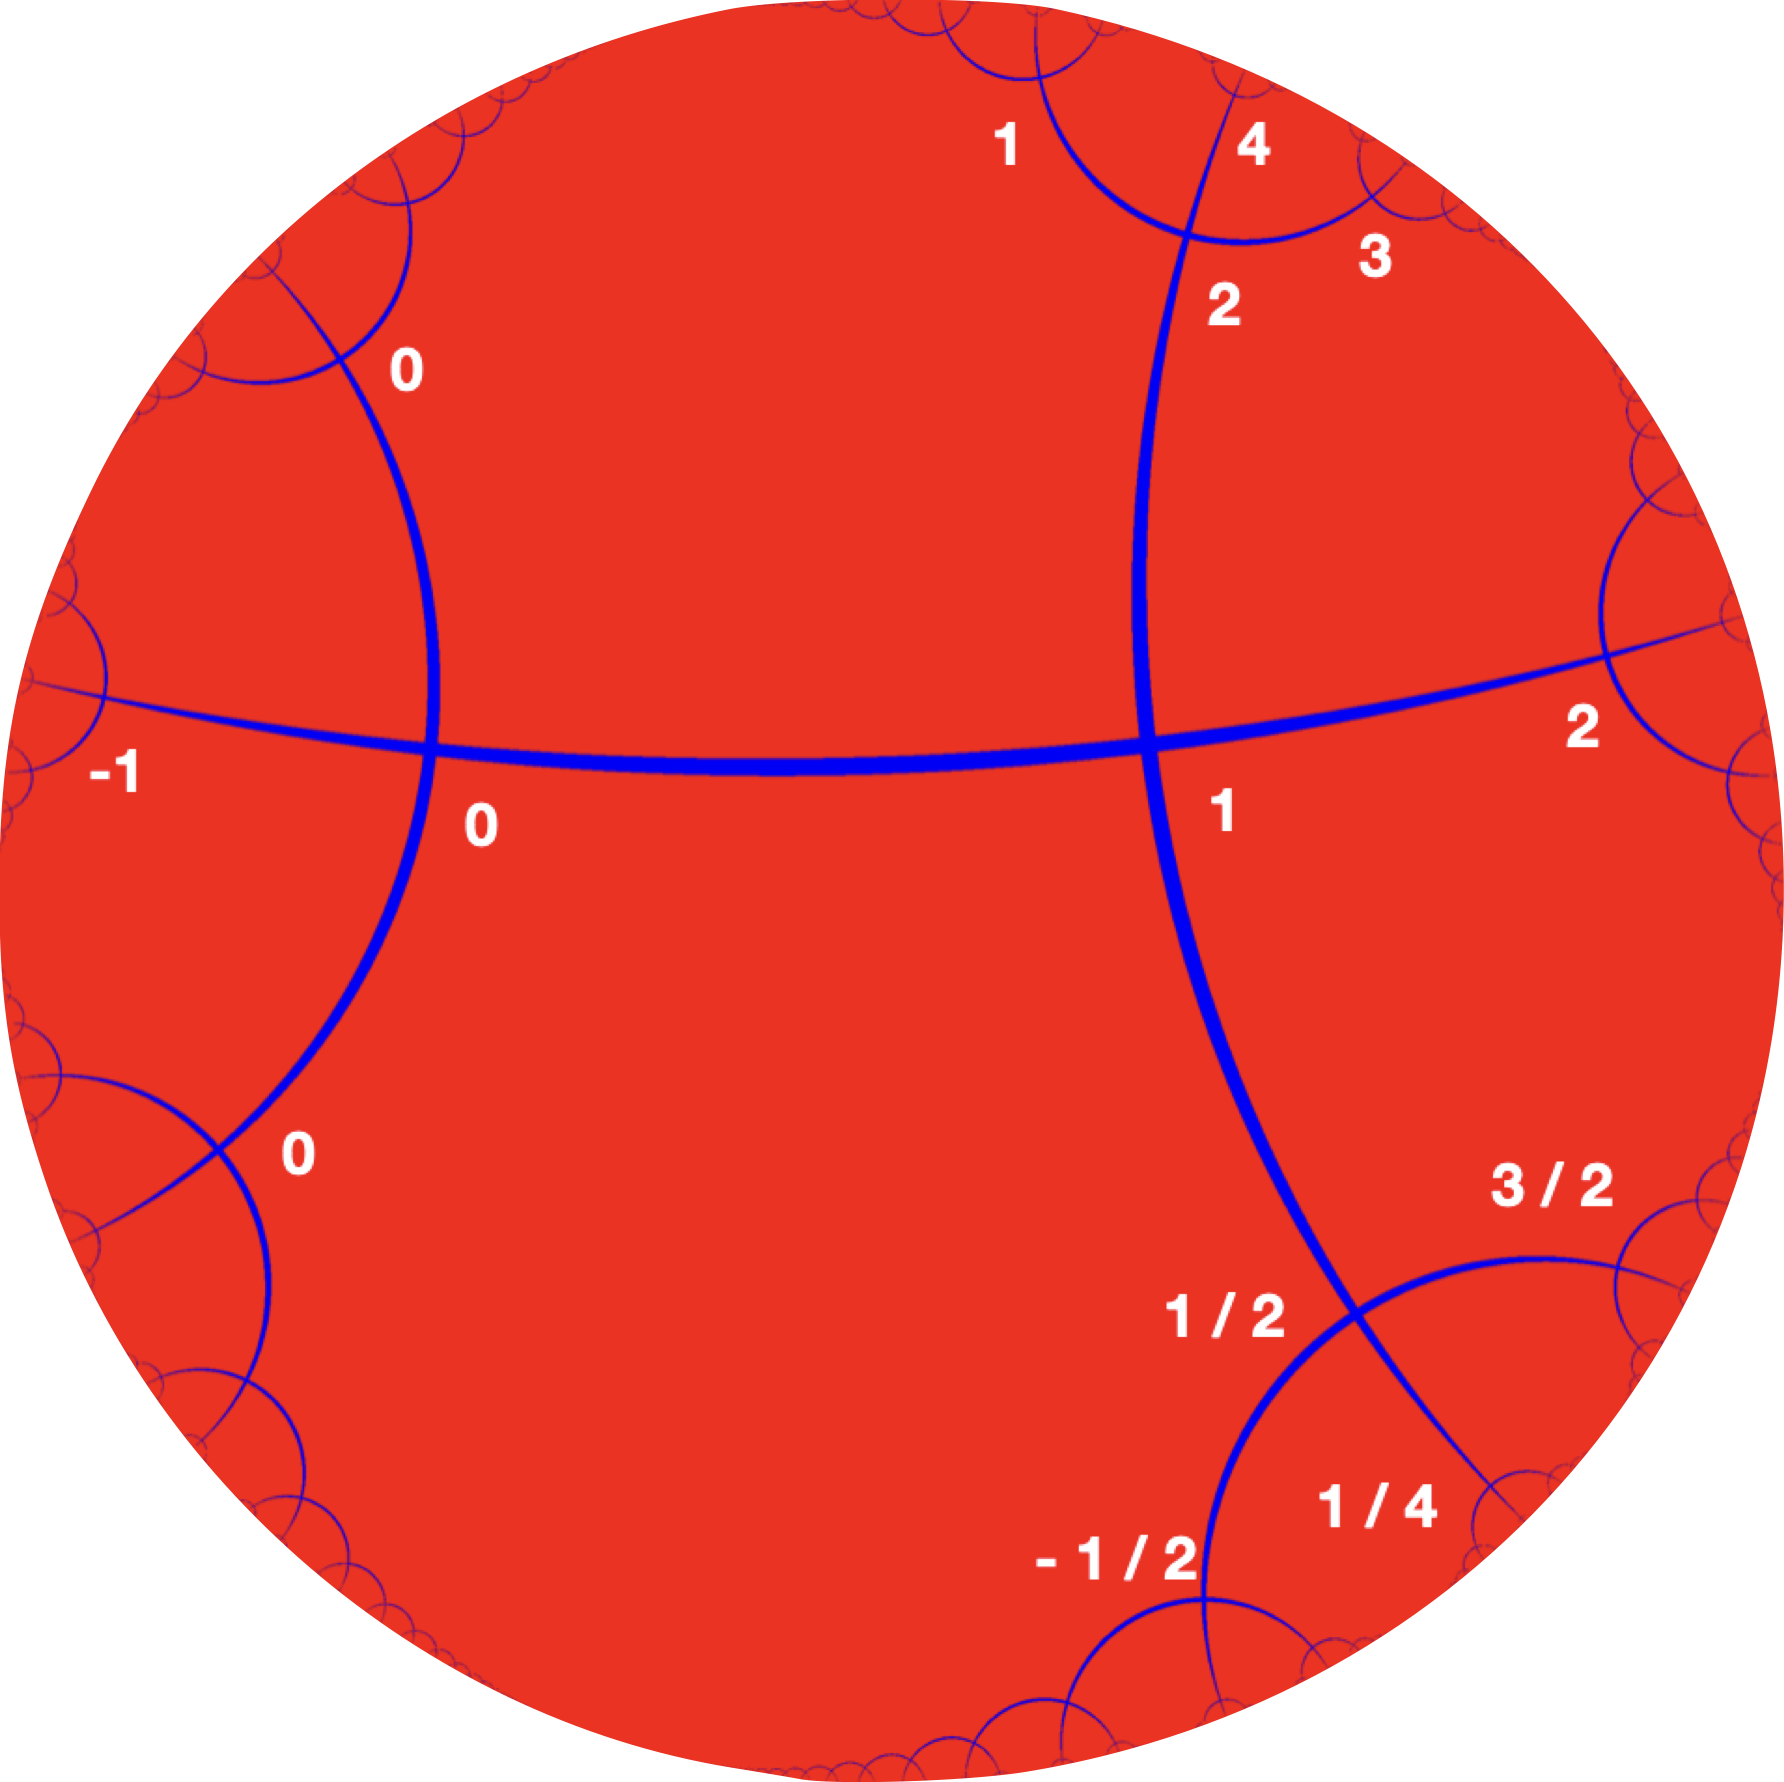
\includegraphics[width=4in]{images/assignment2.png}
\caption{$\cdot + 1$关系、 $\cdot \times 2$关系的赋值网格}
\end{figure}

这个网格的构造规则如下
\begin{enumerate}
    \item 网格呈现为四阶无限边形铺嵌
    \item 加乘轴相互垂直、交替出现
    \item 加轴、乘轴的增长方向按右手系排布
\end{enumerate}

我们可以通过点线面的染色,来论证依照此程序,可以无矛盾的构造几何构形,直至无限边形的无穷远处。

\subsection{流方程的引入}\label{subsec:flow}

假设在一个无穷小范围内存在算术表达式生成结构,它会是什么样呢?本节我们探讨这个话题。
我们假设在赋值 $a_0$ 附近的局部极坐标系下,沿着角度 $\theta$ 有一个运动,经过小时间 $\delta$ 这个运动
在几何上移动了 $\epsilon$,折合到加乘上的变化量,就能导出如下关系

\begin{equation}
    a_{\delta} = (a_0 + \epsilon \cos \theta)e^{\epsilon \sin \theta}
\end{equation}

或者

\begin{equation}
    a_{\delta} = a_0 e^{\epsilon \sin \theta} + \epsilon \cos \theta
\end{equation}

两者都可以简化为

$$
    a_{\delta} = a_0 + \epsilon (a_0 \sin \theta + \cos \theta)
$$

于是

$$
    \frac{1}{\delta} (a_{\delta} - a_0) = \frac{\epsilon}{\delta} (\cos \theta + a_0 \sin \theta)
$$

当 $\delta$ 和 $\epsilon$ 同时趋于零时,我们就得到了 $da / dt$,即有

$$
    \frac{da}{dt} = u (\cos \theta + a \sin \theta)
$$

我们可以改写为其他形式

\begin{equation}
    \frac{da}{ds} = \cos \theta + a \sin \theta \label{eq:flow_1e}
\end{equation}

当 $\theta$ 相对于 $s$ 取常数时,式 \eqref{eq:flow_1e} 对应的微分方程是可解。

\begin{equation}
   a = a_0 e^{s \sin \theta} + (e^{s \sin \theta} - 1) \cot \theta
\end{equation}

上式可以变形为

$$
   a =  a_0 e^{s \sin \theta} + [1 + s \sin \theta + \frac{1}{2!} s\sin^2 \theta  + \frac{1}{3!} s \sin^3 \theta + ... - 1] \cot \theta
$$

进一步有

\begin{equation}
   a =  a_0 e^{s \sin \theta} + s \cos \theta + \frac{1}{2} \sin 2\theta (\frac{s^2}{2!} + \frac{s^3}{3!} \sin \theta + \frac{s^4}{4!} \sin^2 \theta + ...)
   \label{eq:conformance}
\end{equation}

\begin{figure}[ht]
\centering
\begin{tikzpicture}
    \draw (0, 0) node[inner sep=0] {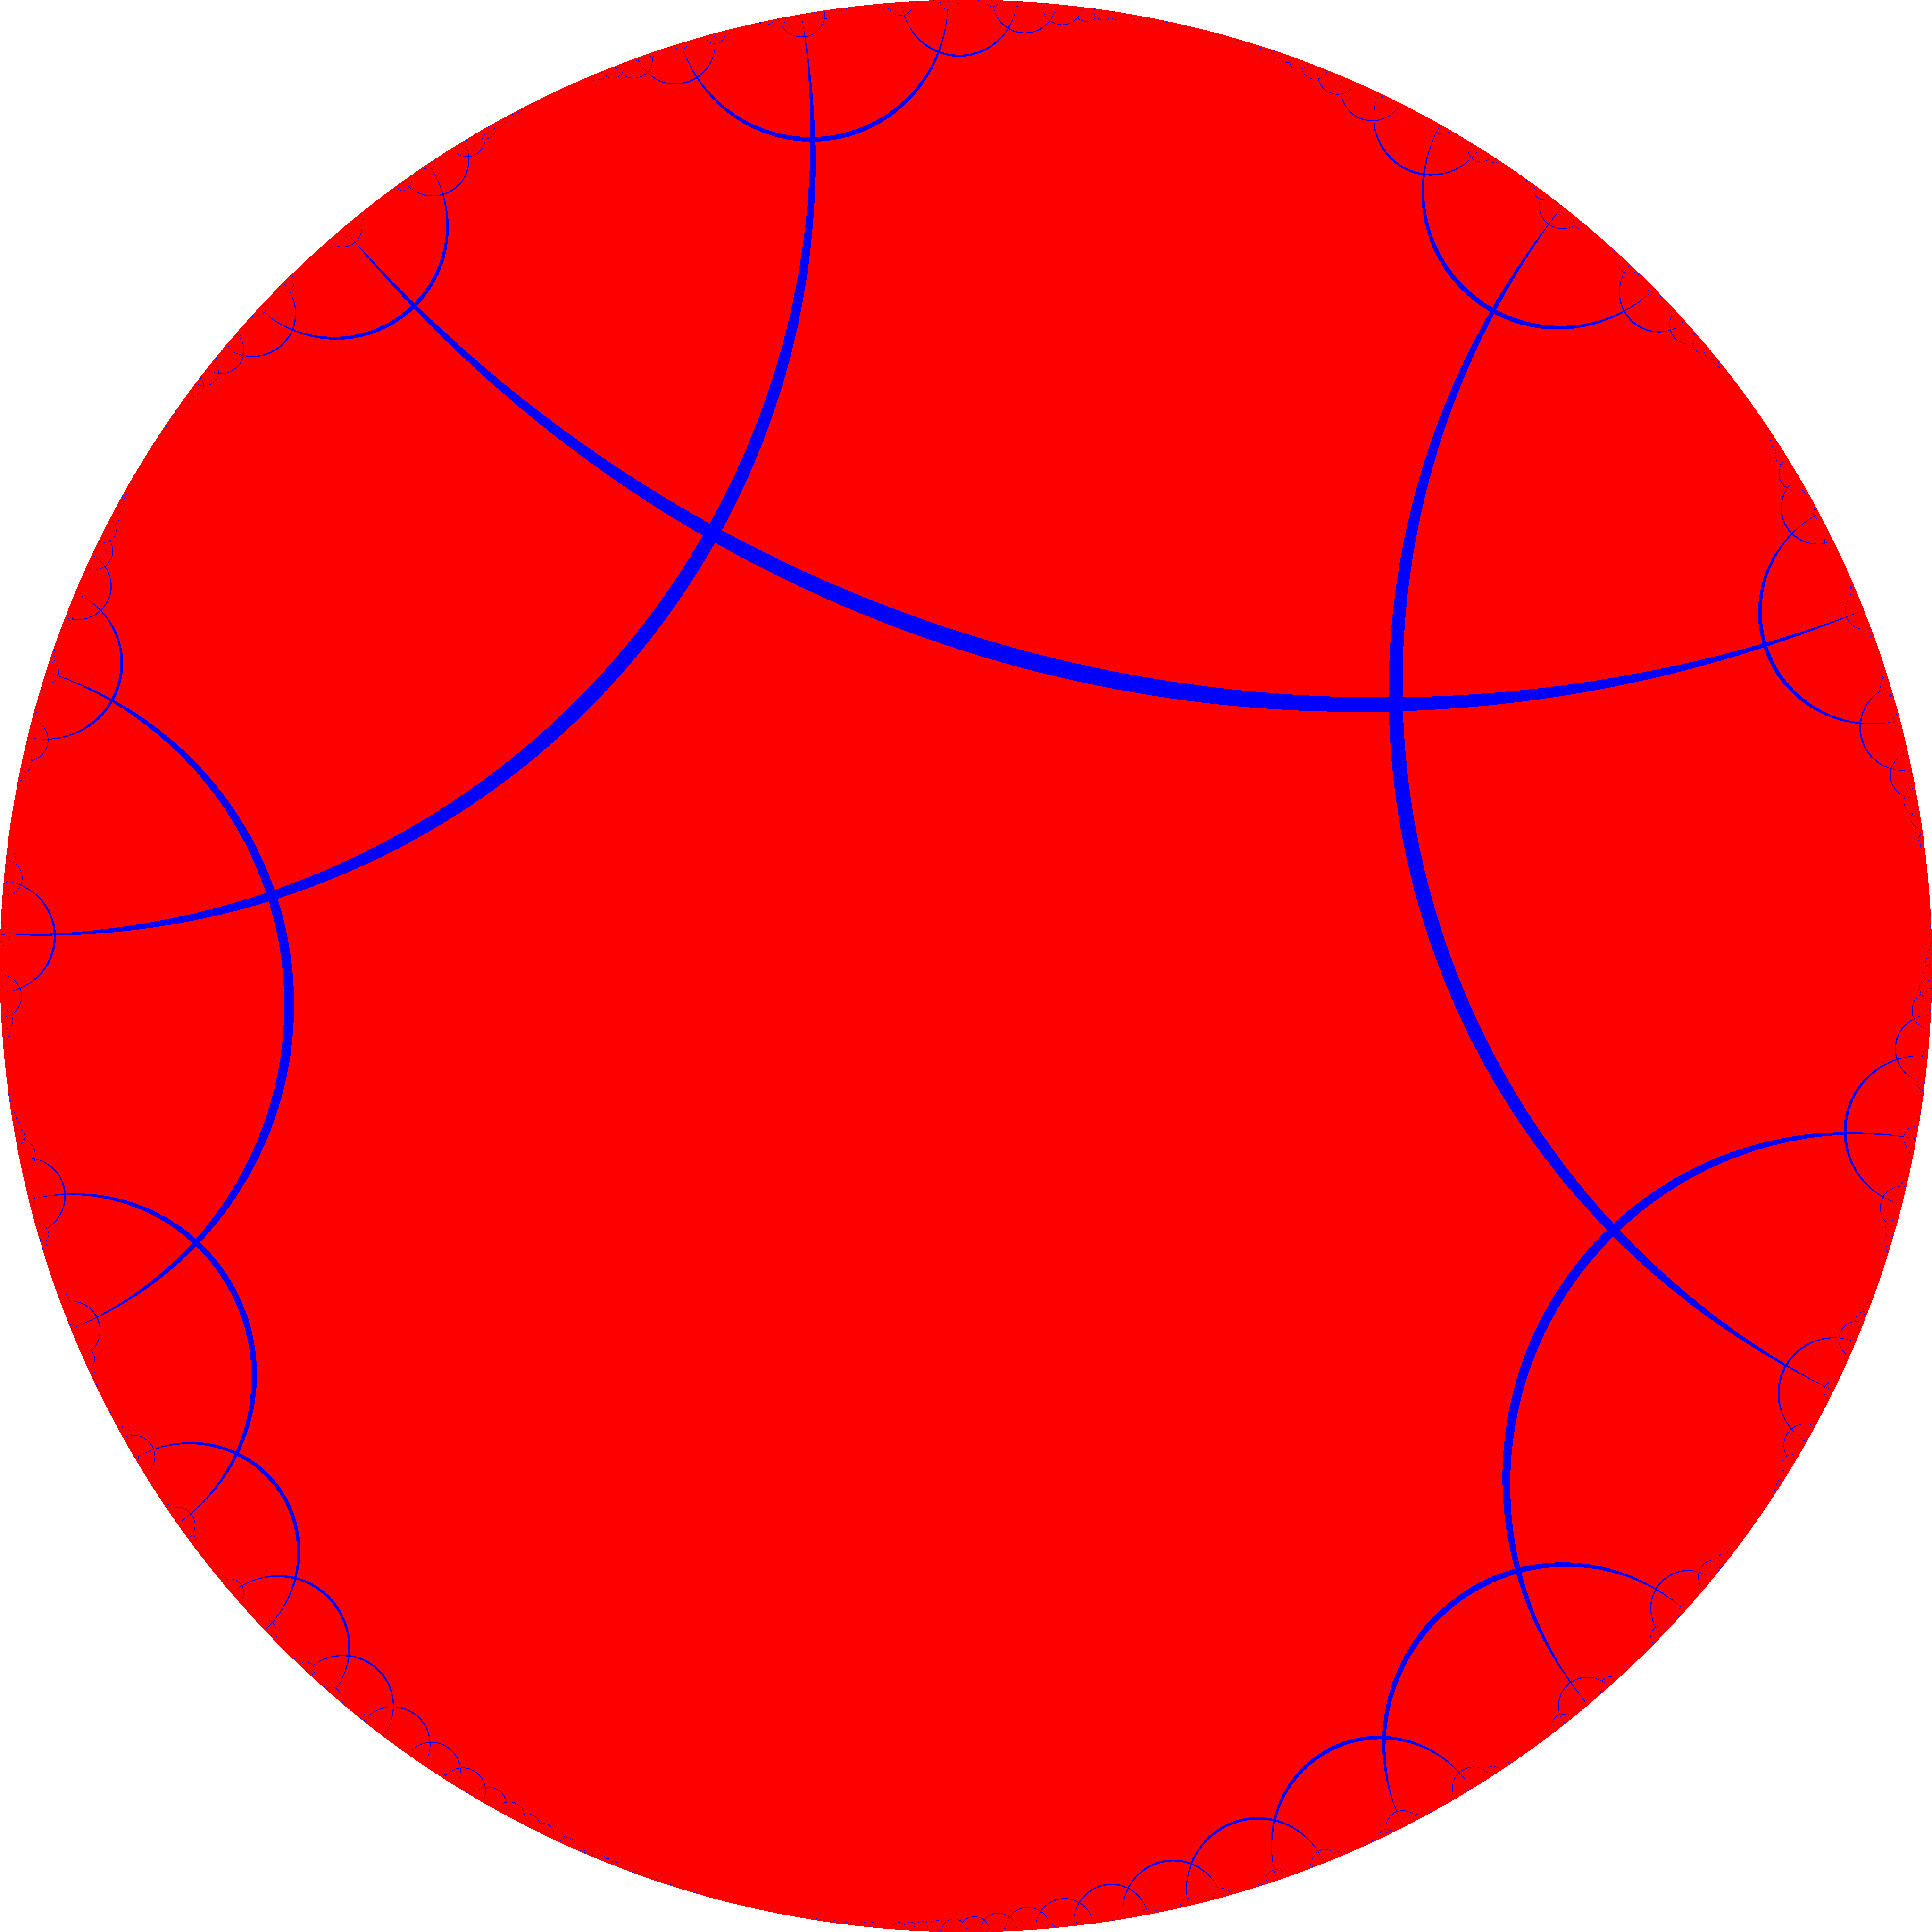
\includegraphics[width=6in]{images/t4096.png}};
    \draw (-4.40, +4.60) node[inner sep=1pt] (s) {$0 - 1$};
    \draw (-2.00, +2.80) node[inner sep=1pt] (z) {$0$};
    \draw (+2.90, +1.60) node[inner sep=1pt] (a) {$0 + 1$};
    \draw (+6.00, +1.60) node[inner sep=1pt] (aa) {$0 + 1 + 1$};
    \draw (+3.00, +5.00) node[inner sep=1pt] (am) {$(0 + 1) \cdot e$};
    \draw (+4.00, -2.00) node[inner sep=1pt] (ad) {$(0 + 1) / e$};
    \draw (-0.80, +6.20) node[inner sep=1pt] (m) {$0 \cdot e$};
    \draw (-4.90, +0.40) node[inner sep=1pt] (d) {$0 / e$};
\end{tikzpicture}
\caption{加乘生成元为 $(1, e)$ 的离散网格}
\label{fig:grid_1e}
\end{figure}

我们把 $ \theta=0, \theta=\pi/2, \theta=\pi, \theta=3\pi/2 $ 代入 \eqref{eq:conformance} 会发现离散网格\ref{fig:grid_1e}和这个解析解是彼此一致的。
即有如下四种情况,

当$ \theta=0, s=1 $ 时:
$$
a =  a_0 + 1
$$

当$ \theta=\pi/2, s=1 $ 时:
$$
a =  a_0 \times e
$$

当$ \theta=\pi, s=1 $ 时:
$$
a =  a_0 - 1
$$

当$ \theta=3\pi/2, s=1 $ 时:
$$
a = a_0 / e
$$

\subsection{更一般的流方程}

我们考察更一般情况下的流方程,假设加法生成元是 $\mu$,乘法生成元是 $\lambda$, 我们可以建立方程

\begin{equation}
    a_{\delta} = (a_0 + \mu \epsilon \cos \theta)e^{\lambda \epsilon \sin \theta}
\end{equation}

或者

\begin{equation}
    a_{\delta} = a_0 e^{\lambda \epsilon \sin \theta} + \mu \epsilon \cos \theta
\end{equation}

两者都可以简化为

\begin{equation}
    a_{\delta} = a_0 + \epsilon (a_0 \lambda \sin \theta + \mu \cos \theta)
\end{equation}

于是

\begin{equation}
    \frac{1}{\delta} (a_{\delta} - a_0) = \frac{\epsilon}{\delta} (\mu \cos \theta + x_0 \lambda \sin \theta)
\end{equation}

当 $\delta$ 和 $\epsilon$ 同时趋于零时,我们就得到了 $da / dt$,即有

\begin{equation}
    \frac{da}{dt} = u (\mu \cos \theta + a \lambda \sin \theta)
\end{equation}

我们可以改写为其他形式

\begin{equation}
    \frac{da}{ds} = \mu \cos \theta + a \lambda \sin \theta\label{eq:flow}
\end{equation}

最后,从式\eqref{eq:flow} 我们能够看到赋值场 $A$ 在度量和角度上的关系,于是得到定理

\begin{theorem}
保距变换保持流方程不变\label{thm:isometry}
\end{theorem}

和上一节一样,流方程形式上是可以解出来,如下:

\begin{equation}
   a =  a_0 e^{\lambda t \sin \theta} + \frac{\mu}{\lambda} (e^{\lambda t \sin \theta} - 1) \cot \theta
\end{equation}

它和离散网格的协调一致性同样可以验证。

\subsection{问题:保方程的变换}

保持流方程不变的充分必要条件仍然还不清晰,可以继续探讨。

\newpage

\section{几个简单实例}

本节我们讨论四个例子,这些例子都可以理解成算术表达式的某种几何表达。
\begin{itemize}
    \item 在几何上,这些例子表现为流形
    \item 在算术上,流形的点都对应算术表达式的某种典范形态
    \item 从表达力的角度讲,任何算术表达式都对应到流形上的一条路径
\end{itemize}

需要声明,本节的陈述是不严密的,“流形的点对应到算术表达式的典范形态”的这个命题仍然需要进一步的严密化。
对第一节实数轴来说,针对实数的严密化手段早已经被戴德金等人发展出来,我们还需要进一步把以往的工作改造成表达式的情形。

\subsection{实数轴的例子}

给定实数轴 $\mathcal{R}$ 和上面的坐标$\phi: \mathcal{R} \to (-\infty, +\infty)$。

\subsubsection{赋值例一}\label{subsec:exmp1}

$\mathcal{R}$ 上 $\phi$ 取值为有理数的全体点构成集合 $Q$,而 $Q$ 中的每个点都有$b$-进数位制下的表示,
从而 $Q$ 也可以理解成有限长度的典范算术表达式的集合,这些表达式均具如下形式:
$$
\sum_{i} k_i b^{l_i}, k_i \in N, l_i \in N
$$

$Q$ 作为数可以完备化得到实数全体 $(-\infty, +\infty)$,而类似的完备化过程也可以把有限长度的典范算术表达式
扩展到无限长度的典范算术表达式。

\subsection{上半平面模型下的例子\footnote{本例子的解析解由张乐给出,几何和典范形式的解释由笔者给出。}}

考虑上半平面
\[
\{\mathcal{H}: (x, y) | y > 0 \}
\]

配有如下的内积

\[
\mathbf{a} \cdot \mathbf{b} = \begin{bmatrix} a_x & a_y \end{bmatrix} \begin{bmatrix} \frac{1}{y^2} & 0 \\ 0 & \frac{1}{y^2} \end{bmatrix} \begin{bmatrix} b_x \\ b_y \end{bmatrix}
\]

以及度规

\[
ds^2 = \frac{dx^2 + dy^2}{y^2}
\]

这个流形的高斯曲率是 $-1$,并有 Laplacian 为

\[
\Delta = - y^2 (\frac{\partial^2}{\partial x^2} + \frac{\partial^2}{\partial y^2})
\]

\subsubsection{赋值例二}\label{subsec:exmp2}

给定一个赋值函数

\begin{equation}
A = - \frac{x}{y}
\end{equation}

首先,我们可以验证,在每个局域,$A$ 满足流方程。

\begin{theorem}\footnote{本证明思路由张乐给出,略作改动。}
如上定义的 $A$ 满足流方程
\end{theorem}

\begin{proof}
$$
da = d(-\frac{x}{y}) = \frac{xdy - ydx}{y^2} = -\frac{dx + ady}{y}
$$

注意到

$$
ds = \frac{\sqrt{dx^2 + dy^2}}{y}
$$

便有

$$
\frac{da}{ds} = - \frac{dx + ady}{y} \frac{y}{\sqrt{dx^2 + dy^2}} = - \frac{dx + ady}{\sqrt{dx^2 + dy^2}}
$$

考虑到局部坐标由 $(-1, 0)$ 和 $(0, -1)$ 依照右手螺旋给出,就有

$$
\cos \theta = \frac{\begin{bmatrix} dx & dy \end{bmatrix} \begin{bmatrix} \frac{1}{y^2} & 0 \\ 0 & \frac{1}{y^2} \end{bmatrix} \begin{bmatrix} -1 \\ 0 \end{bmatrix}}{\sqrt{\begin{bmatrix} dx & dy \end{bmatrix} \begin{bmatrix} \frac{1}{y^2} & 0 \\ 0 & \frac{1}{y^2} \end{bmatrix} \begin{bmatrix} dx \\ dy \end{bmatrix}}\sqrt{\begin{bmatrix} -1 & 0 \end{bmatrix} \begin{bmatrix} \frac{1}{y^2} & 0 \\ 0 & \frac{1}{y^2} \end{bmatrix} \begin{bmatrix} -1 \\ 0 \end{bmatrix}}}
$$

即有

$$
\cos \theta = \frac{-dx}{\sqrt{dx^2 + dy^2}}
$$

类似有

$$
\sin \theta = \frac{-dy}{\sqrt{dx^2 + dy^2}}
$$

于是有

$$
\frac{da}{ds} = \cos \theta + a \sin \theta
$$

\end{proof}

\subsubsection{Laplacian 的特征向量}

我们可以验证 $A$ 是 Laplacian 的特征向量。

$$
\Delta A = - y^2 (\frac{\partial^2}{\partial x^2} A + \frac{\partial^2}{\partial y^2} A) = y^2 (\frac{1}{\partial y} (\frac{1}{\partial y} \frac{x}{y})) = 2 A
$$

\subsection{伪圆坐标系下的两个例子\footnote{本例子的解析解由张乐给出,几何和典范形式的解释由笔者给出。}}

首先介绍双曲空间的伪圆坐标系。伪圆坐标系是利用一族伪圆和与之正交的测地线族来定位的全局坐标系统。
如图所示,在红色的庞加莱圆盘$\mathcal{P}$上,蓝色的伪圆相切于理想点 $\Omega$,绿线是与之正交的测地线。
那么点 $P$ 的坐标由 $QP$ 和 $OQ$ 的有向长度给出,点 $O$ 为坐标原点,有向长度都是双曲空间内的长度。
在测地线族上有向长度的正负号,根据点 $P$ 是否在 $\Omega$ 点一侧来确定,在 $\Omega$ 点一侧为正,否则为负。
在伪圆族上有向长度的正负号,按照右手螺旋为增加的方向来确定,也即右手螺旋过点 $O$ 相继给出了负半轴和正半轴。
依照如上规则,点 $P$ 的坐标为 $(x,y)$。

\begin{figure}[ht]
\centering
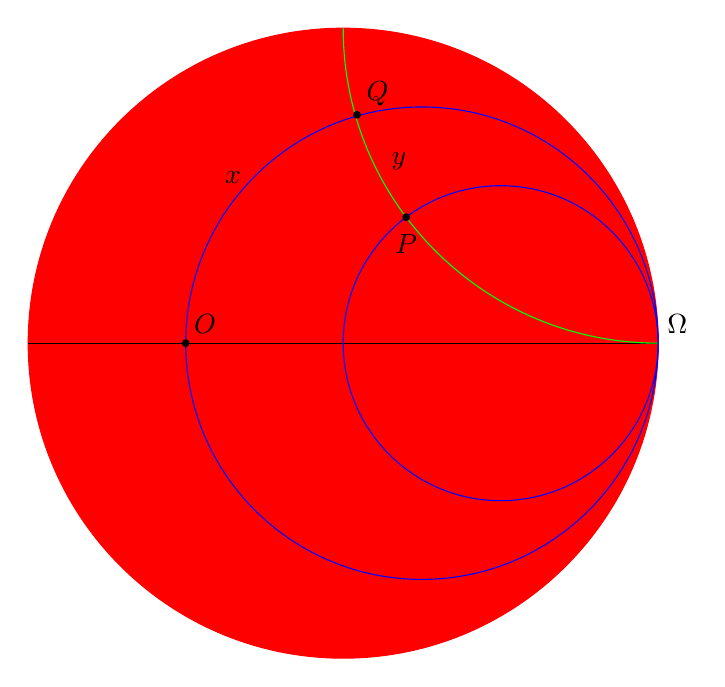
\begin{tikzpicture}
    \node[anchor=225] at (4,2) {$\Omega$};
    \draw[red,fill=red] (0,2) circle[radius=4];
    \draw[blue] (1, 2) circle[radius=3];
    \draw[black] (-4,2) -- (4,2);
    \draw[green] (4,2) arc (-90:-180:4);
    \draw[blue] (2, 2) circle[radius=2];
    \node[fill,circle,inner sep=1pt] at (-2,2) {};
    \node[anchor=225] at (-2,2) {$O$};
    \node[fill,circle,inner sep=1pt] at (0.175,4.9) {};
    \node[anchor=225] at (0.175,4.9) {$Q$};
    \node[fill,circle,inner sep=1pt] at (0.8,3.6) {};
    \node[anchor=90] at (0.8,3.5) {$P$};
    \node[anchor=225] at (0.49,4.1) {$y$};
    \node[anchor=225] at (-1.6,3.9) {$x$};
\end{tikzpicture}
\caption{伪圆坐标系}\label{fig:horocyclecoord}
\end{figure}

我们有

$$
ds^2 = e^{-2y} dx^2 + dy^2
$$

和

$$
\Delta = e^{2y} \frac{\partial^2}{{\partial x}^2} + \frac{\partial^2}{{\partial y}^2} - \frac{\partial}{\partial y}
$$

\subsubsection{赋值例三}\label{subsec:exmp3}

伪圆坐标系下的第一个例子是

\begin{equation}
A = x e^{-y}
\end{equation}

\begin{figure}[ht]
\centering
\begin{tikzpicture}
\draw [black, line width=0.6pt, ->] (0,0) to[out=90,in=270] (0,4.25);
\node [anchor=south] at (0,4.5) {y};
\draw [black, line width=0.6pt, ->] (-4.25,0) to[out=0,in=180] (4.25,0);
\node [anchor=west] at (4.5,0) {x};

\draw [blue, line width=0.6pt] (-4.25,4.0) to[out=0,in=180] (4.25,4.0);
\draw [blue, line width=0.6pt] (-4.25,2.0) to[out=0,in=180] (4.25,2.0);
\draw [green, line width=0.6pt] (-3.5,0) to[out=90,in=270] (-3.5,4.5);

\node[anchor=45] at (0.0,4.0) {$O$};
\node[anchor=45] at (-3.5,4.0) {$Q$};
\node[anchor=45] at (-3.5,2.0) {$P$};
\node[anchor=225] at (-2.0,4.1) {$x = u$};
\node[anchor=225] at (-3.0,1.0) {$y = e^v$};

\end{tikzpicture}

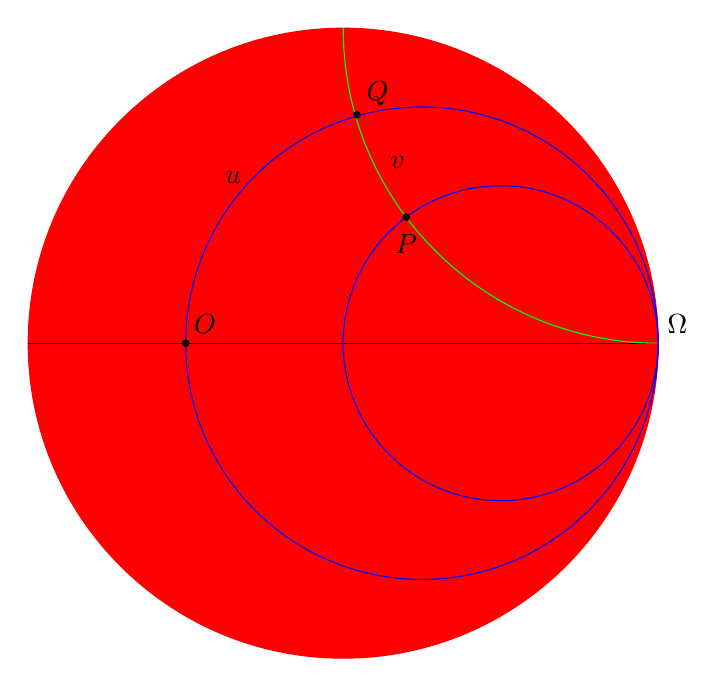
\begin{tikzpicture}
    \node[anchor=225] at (4,2) {$\Omega$};
    \draw[red,fill=red] (0,2) circle[radius=4];
    \draw[blue] (1, 2) circle[radius=3];
    \draw[black] (-4,2) -- (4,2);
    \draw[green] (4,2) arc (-90:-180:4);
    \draw[blue] (2, 2) circle[radius=2];
    \node[fill,circle,inner sep=1pt] at (-2,2) {};
    \node[anchor=225] at (-2,2) {$O$};
    \node[fill,circle,inner sep=1pt] at (0.175,4.9) {};
    \node[anchor=225] at (0.175,4.9) {$Q$};
    \node[fill,circle,inner sep=1pt] at (0.8,3.6) {};
    \node[anchor=90] at (0.8,3.5) {$P$};
    \node[anchor=225] at (0.49,4.1) {$v$};
    \node[anchor=225] at (-1.6,3.9) {$u$};
\end{tikzpicture}
\caption{例二和例三之间的映射}\label{fig:mapping}
\end{figure}

\begin{proof}

针对上一个例子里的设定 \ref{subsec:exmp2},我们引入复数

$$
z = x + y i
$$

而如下的 Möbius 变换

$$
z \mapsto \frac{z-i}{z+i}
$$

可以把前例 \ref{subsec:exmp2} 里的上半平面模型变到当前的伪圆坐标系。

这个变换把 $\mathcal{H}$ 里的每一条横线变成 $\mathcal{P}$ 里过理想点 $\Omega = 1$的伪圆。
把 $\mathcal{H}$ 里的每一条竖测地线变成 $\mathcal{P}$ 里和上述伪圆族垂直的测地线。

不难得到如下的坐标变换公式:

$$
\begin{cases}
x = u\\
y = e^v \\
\end{cases}
$$

因此有

$$
A = -\frac{x}{y} = u e^{-v}
$$

根据定理\ref{thm:isometry} 以及 Möbius 变换共形,我们可以得到 $A = u e^{-v}$ 遵守流方程。

\end{proof}

此时,有

$$
\Delta A = e^{2y} \frac{\partial^2(x e^{-y})}{{\partial x}^2} + \frac{\partial^2(x e^{-y})}{{\partial y}^2} - \frac{\partial(x e^{-y})}{\partial y} = 2A
$$

\subsubsection{赋值例四}\label{subsec:exmp4}

伪圆坐标系下的第二个例子是

\begin{equation}
A = x e^y
\end{equation}

注意到例子三和例子四也可以通过共形变联系起来,由如下映射给出

$$
(x, y) \mapsto (x, -y)
$$

因此例子四也满足流方程。

注意到此时 $A$ 在边界上趋于 $0$ 值,同时有

$$
\Delta A = e^{2y} \frac{\partial^2(x e^y)}{{\partial x}^2} + \frac{\partial^2(x e^y)}{{\partial y}^2} - \frac{\partial(x e^y)}{\partial y} = 0
$$

\subsection{几个问题}

\subsubsection{例子和方程解的融洽}

以上四个例子都是给定的全局坐标系,而流方程的形式解是在局部坐标系下给出的,两者是否融洽,是一个可以考察的问题。
这里面可能不只是涉及坐标变换,也可能还有几何上的黏合与复叠。

\newpage

\section{任意生成元的例子}

本节我们将会给出赋值的第五个例子。在这个例子里,我们会看到赋值和生成元的具体取值无关;同时,我们在同一个底图上采用了不同的生成元,
都能够画出来一些很匀称的网格。我们将研究这些网格的几何含义,并在赋值和网格的基础上,导出第五个例子中的算术表达式的典范形态。

考虑上半平面
\[
\{\mathcal{B}: (x, y) | y > 0 \}
\]

配有如下的内积

\[
\mathbf{a} \cdot \mathbf{b} = \begin{bmatrix} a_x & a_y \end{bmatrix} \begin{bmatrix} \frac{1}{\mu^2 y^2} & 0 \\ 0 & \frac{1}{\lambda^2 y^2} \end{bmatrix} \begin{bmatrix} b_x \\ b_y \end{bmatrix}
\]

以及度规

\[
ds^2 = \frac{1}{y^2}(\frac{dx^2}{\mu^2} + \frac{dy^2}{\lambda^2})
\]

\subsection{赋值例五}\label{subsec:exmp5}

给定一个赋值函数

\begin{equation}
A = - \frac{x}{y}
\end{equation}

我们可以验证,在每个局域,$A$ 满足流方程。

\begin{theorem}
如上定义的 $A$ 满足流方程
\end{theorem}

\begin{proof}
$$
da = d(-\frac{x}{y}) = \frac{xdy - ydx}{y^2} = -\frac{dx + a dy}{y}
$$

注意到

$$
ds = \frac{1}{y}\sqrt{\frac{dx^2}{\mu^2} + \frac{dy^2}{\lambda^2}}
$$

便有

$$
\frac{da}{ds} = - \frac{dx + a dy}{y} \frac{y}{\sqrt{\frac{dx^2}{\mu^2} + \frac{dy^2}{\lambda^2}}} = \frac{dx + a dy}{\sqrt{\frac{dx^2}{\mu^2} + \frac{dy^2}{\lambda^2}}}
$$

考虑到局部坐标由 $(-1, 0)$ 和 $(0, -1)$ 依照右手螺旋给出,就有

$$
\cos \theta = \frac{\begin{bmatrix} dx & dy \end{bmatrix} \begin{bmatrix} \frac{1}{\mu^2 y^2} & 0 \\ 0 & \frac{1}{\lambda^2 y^2} \end{bmatrix} \begin{bmatrix} -1 \\ 0 \end{bmatrix}}{\sqrt{\begin{bmatrix} dx & dy \end{bmatrix} \begin{bmatrix} \frac{1}{\mu^2 y^2} & 0 \\ 0 & \frac{1}{\lambda^2 y^2} \end{bmatrix} \begin{bmatrix} dx \\ dy \end{bmatrix}}\sqrt{\begin{bmatrix} -1 & 0 \end{bmatrix} \begin{bmatrix} \frac{1}{\mu^2 y^2} & 0 \\ 0 & \frac{1}{\lambda^2 y^2} \end{bmatrix} \begin{bmatrix} -1 \\ 0 \end{bmatrix}}}
$$

即有

$$
\cos \theta = \frac{-\frac{dx}{\mu}}{\sqrt{\frac{dx^2}{\mu^2} + \frac{dy^2}{\lambda^2}}}
$$

类似有

$$
\sin \theta = \frac{-\frac{dy}{\lambda}}{\sqrt{\frac{dx^2}{\mu^2} + \frac{dy^2}{\lambda^2}}}
$$

于是有

$$
\frac{da}{ds} = \mu \cos \theta + a \lambda \sin \theta
$$

\end{proof}

例五的赋值 $A$ 与生成元的具体取值无关。

\subsection{网格的构造}

对不同的生成元,它们都共享一条基础的加线和一条基础的乘线。
\begin{itemize}
    \item 基础的加线: $y = 1$
    \item 基础的乘线: $x = 0$,整条线是一条零线
\end{itemize}

\subsubsection{网格例一}

在网格例一里,蓝线代表 $+ 1$ 关系,绿线代表 $\times 2$ 关系,它们是彼此垂直的线族。

\begin{figure}[ht]
\centering
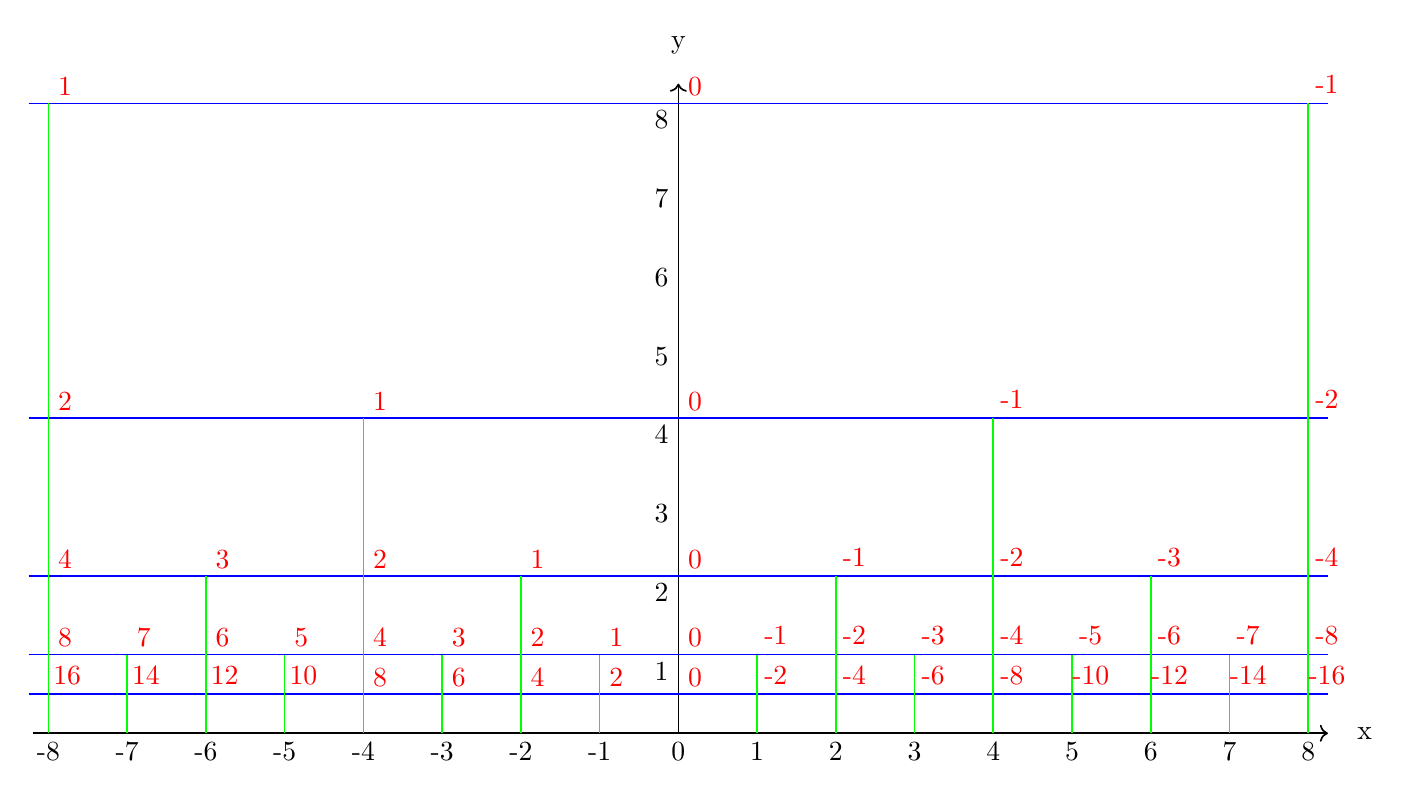
\begin{tikzpicture}
\draw [black, line width=0.6pt, ->] (0,0) to[out=90,in=270] (0,8.25);
\node [anchor=south] at (0,8.5) {y};
\draw [black, line width=0.6pt, ->] (-8.2,0) to[out=0,in=180] (8.25,0);
\node [anchor=west] at (8.5,0) {x};
\foreach \x in {-8,-7,-6,-5,-4,-3,-2,-1,0,1,2,3,4,5,6,7,8}
  \node [anchor=north] at (\x,0) {\x};
\foreach \y in {1,2,3,4,5,6,7,8}
  \node [anchor=45] at (0,\y) {\y};

\draw [blue, line width=0.6pt] (-8.25,0.5) to[out=0,in=180] (8.25,0.5);
\draw [blue, line width=0.6pt] (-8.25,1) to[out=0,in=180] (8.25,1);
\draw [blue, line width=0.6pt] (-8.25,2) to[out=0,in=180] (8.25,2);
\draw [blue, line width=0.6pt] (-8.25,4) to[out=0,in=180] (8.25,4);
\draw [blue, line width=0.6pt] (-8.25,8) to[out=0,in=180] (8.25,8);

\draw [green, line width=0.6pt] (-8,0) to[out=90,in=270] (-8,1);
\draw [green, line width=0.6pt] (-7,0) to[out=90,in=270] (-7,1);
\draw [green, line width=0.6pt] (-6,0) to[out=90,in=270] (-6,1);
\draw [green, line width=0.6pt] (-5,0) to[out=90,in=270] (-5,1);
\draw [green, line width=0.6pt] (-4,0) to[out=90,in=270] (-4,1);
\draw [green, line width=0.6pt] (-3,0) to[out=90,in=270] (-3,1);
\draw [green, line width=0.6pt] (-2,0) to[out=90,in=270] (-2,1);
\draw [green, line width=0.6pt] (-1,0) to[out=90,in=270] (-1,1);
\draw [green, line width=0.6pt] (1,0) to[out=90,in=270] (1,1);
\draw [green, line width=0.6pt] (2,0) to[out=90,in=270] (2,1);
\draw [green, line width=0.6pt] (3,0) to[out=90,in=270] (3,1);
\draw [green, line width=0.6pt] (4,0) to[out=90,in=270] (4,1);
\draw [green, line width=0.6pt] (5,0) to[out=90,in=270] (5,1);
\draw [green, line width=0.6pt] (6,0) to[out=90,in=270] (6,1);
\draw [green, line width=0.6pt] (7,0) to[out=90,in=270] (7,1);
\draw [green, line width=0.6pt] (8,0) to[out=90,in=270] (8,1);

\draw [green, line width=0.6pt] (-8,1) to[out=90,in=270] (-8,2);
\draw [green, line width=0.6pt] (-6,1) to[out=90,in=270] (-6,2);
\draw [green, line width=0.6pt] (-4,1) to[out=90,in=270] (-4,2);
\draw [green, line width=0.6pt] (-2,1) to[out=90,in=270] (-2,2);
\draw [green, line width=0.6pt] (2,1) to[out=90,in=270] (2,2);
\draw [green, line width=0.6pt] (4,1) to[out=90,in=270] (4,2);
\draw [green, line width=0.6pt] (6,1) to[out=90,in=270] (6,2);
\draw [green, line width=0.6pt] (8,1) to[out=90,in=270] (8,2);

\draw [green, line width=0.6pt] (-8,2) to[out=90,in=270] (-8,4);
\draw [green, line width=0.6pt] (-4,2) to[out=90,in=270] (-4,4);
\draw [green, line width=0.6pt] (4,2) to[out=90,in=270] (4,4);
\draw [green, line width=0.6pt] (8,2) to[out=90,in=270] (8,4);

\draw [green, line width=0.6pt] (-8,4) to[out=90,in=270] (-8,8);
\draw [green, line width=0.6pt] (8,4) to[out=90,in=270] (8,8);

\node [anchor=225, red] at (-8,0.5) {16};
\node [anchor=225, red] at (-7,0.5) {14};
\node [anchor=225, red] at (-6,0.5) {12};
\node [anchor=225, red] at (-5,0.5) {10};
\node [anchor=225, red] at (-4,0.5) {8};
\node [anchor=225, red] at (-3,0.5) {6};
\node [anchor=225, red] at (-2,0.5) {4};
\node [anchor=225, red] at (-1,0.5) {2};
\node [anchor=225, red] at (0,0.5) {0};
\node [anchor=225, red] at (1,0.5) {-2};
\node [anchor=225, red] at (2,0.5) {-4};
\node [anchor=225, red] at (3,0.5) {-6};
\node [anchor=225, red] at (4,0.5) {-8};
\node [anchor=225, red] at (5,0.5) {-10};
\node [anchor=225, red] at (6,0.5) {-12};
\node [anchor=225, red] at (7,0.5) {-14};
\node [anchor=225, red] at (8,0.5) {-16};

\node [anchor=225, red] at (-8,1) {8};
\node [anchor=225, red] at (-7,1) {7};
\node [anchor=225, red] at (-6,1) {6};
\node [anchor=225, red] at (-5,1) {5};
\node [anchor=225, red] at (-4,1) {4};
\node [anchor=225, red] at (-3,1) {3};
\node [anchor=225, red] at (-2,1) {2};
\node [anchor=225, red] at (-1,1) {1};
\node [anchor=225, red] at (0,1) {0};
\node [anchor=225, red] at (1,1) {-1};
\node [anchor=225, red] at (2,1) {-2};
\node [anchor=225, red] at (3,1) {-3};
\node [anchor=225, red] at (4,1) {-4};
\node [anchor=225, red] at (5,1) {-5};
\node [anchor=225, red] at (6,1) {-6};
\node [anchor=225, red] at (7,1) {-7};
\node [anchor=225, red] at (8,1) {-8};

\node [anchor=225, red] at (-8,2) {4};
\node [anchor=225, red] at (-6,2) {3};
\node [anchor=225, red] at (-4,2) {2};
\node [anchor=225, red] at (-2,2) {1};
\node [anchor=225, red] at (0,2) {0};
\node [anchor=225, red] at (2,2) {-1};
\node [anchor=225, red] at (4,2) {-2};
\node [anchor=225, red] at (6,2) {-3};
\node [anchor=225, red] at (8,2) {-4};

\node [anchor=225, red] at (-8,4) {2};
\node [anchor=225, red] at (-4,4) {1};
\node [anchor=225, red] at (0,4) {0};
\node [anchor=225, red] at (4,4) {-1};
\node [anchor=225, red] at (8,4) {-2};

\node [anchor=225, red] at (-8,8) {1};
\node [anchor=225, red] at (0,8) {0};
\node [anchor=225, red] at (8,8) {-1};

\end{tikzpicture}
\caption{网格例一,$\lambda=\ln2$ 和 $\mu=1$}\label{fig:gridex1}
\end{figure}

\subsubsection{网格例二}

在网格例二里,蓝线代表 $+ 1$ 关系,绿线代表 $\times 3$ 关系,它们是彼此垂直的线族。

\begin{figure}[ht]
\centering
\resizebox{\columnwidth}{!}{%
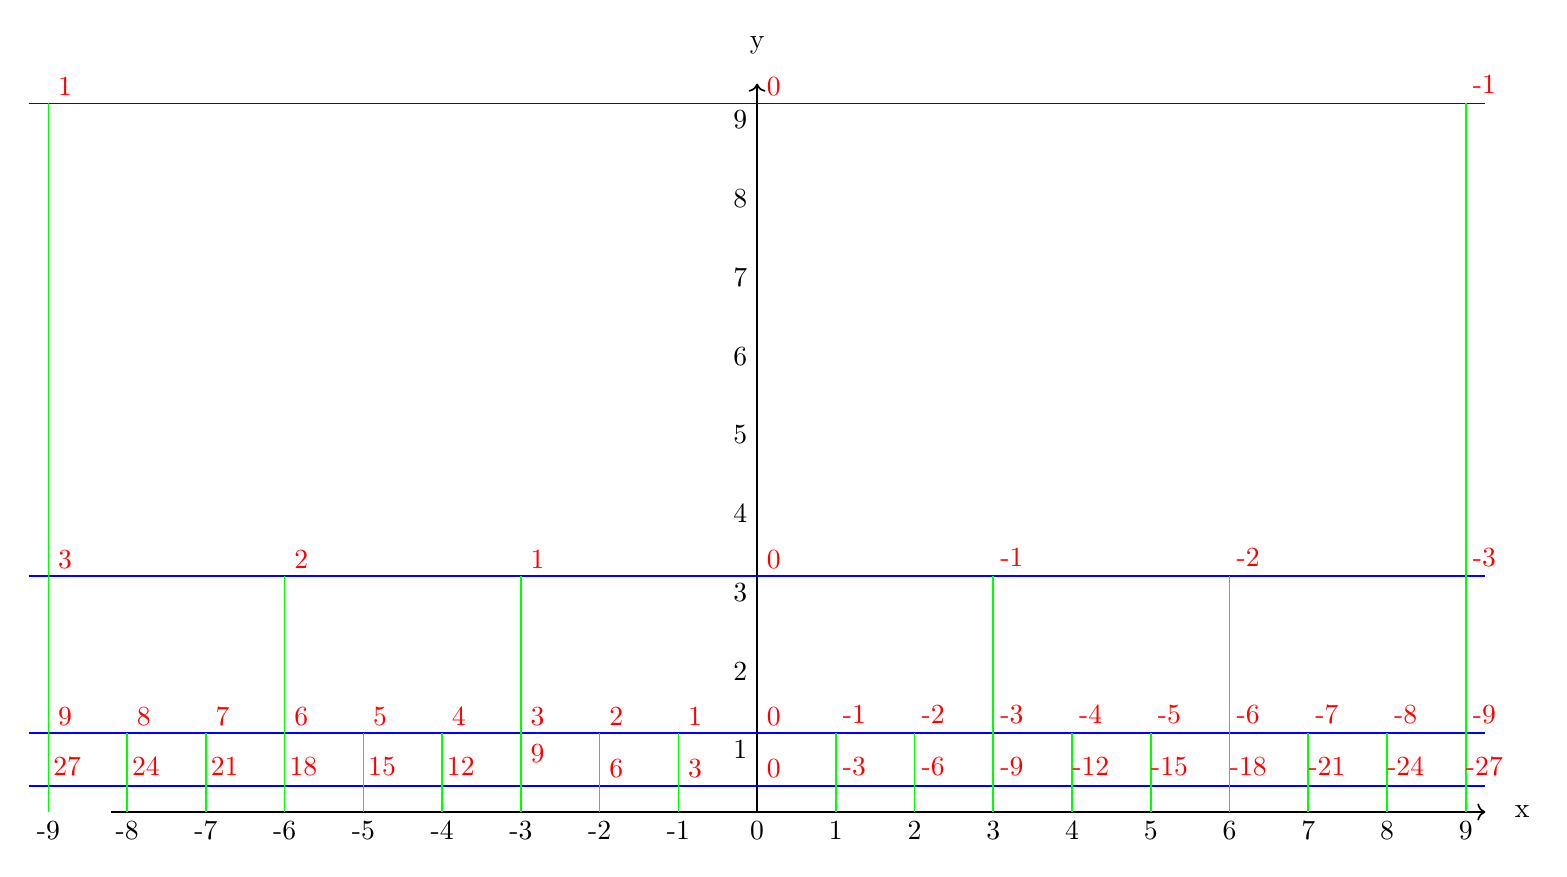
\begin{tikzpicture}
\draw [black, line width=0.6pt, ->] (0,0) to[out=90,in=270] (0,9.25);
\node [anchor=south] at (0,9.5) {y};
\draw [black, line width=0.6pt, ->] (-8.2,0) to[out=0,in=180] (9.25,0);
\node [anchor=west] at (9.5,0) {x};
\foreach \x in {-9,-8,-7,-6,-5,-4,-3,-2,-1,0,1,2,3,4,5,6,7,8,9}
  \node [anchor=north] at (\x,0) {\x};
\foreach \y in {1,2,3,4,5,6,7,8,9}
  \node [anchor=45] at (0,\y) {\y};

\draw [blue, line width=0.6pt] (-9.25,0.3333) to[out=0,in=180] (9.25,0.3333);
\draw [blue, line width=0.6pt] (-9.25,1) to[out=0,in=180] (9.25,1);
\draw [blue, line width=0.6pt] (-9.25,3) to[out=0,in=180] (9.25,3);
\draw [blue, line width=0.6pt] (-9.25,9) to[out=0,in=180] (9.25,9);

\draw [green, line width=0.6pt] (-9,0) to[out=90,in=270] (-9,1);
\draw [green, line width=0.6pt] (-8,0) to[out=90,in=270] (-8,1);
\draw [green, line width=0.6pt] (-7,0) to[out=90,in=270] (-7,1);
\draw [green, line width=0.6pt] (-6,0) to[out=90,in=270] (-6,1);
\draw [green, line width=0.6pt] (-5,0) to[out=90,in=270] (-5,1);
\draw [green, line width=0.6pt] (-4,0) to[out=90,in=270] (-4,1);
\draw [green, line width=0.6pt] (-3,0) to[out=90,in=270] (-3,1);
\draw [green, line width=0.6pt] (-2,0) to[out=90,in=270] (-2,1);
\draw [green, line width=0.6pt] (-1,0) to[out=90,in=270] (-1,1);
\draw [green, line width=0.6pt] (1,0) to[out=90,in=270] (1,1);
\draw [green, line width=0.6pt] (2,0) to[out=90,in=270] (2,1);
\draw [green, line width=0.6pt] (3,0) to[out=90,in=270] (3,1);
\draw [green, line width=0.6pt] (4,0) to[out=90,in=270] (4,1);
\draw [green, line width=0.6pt] (5,0) to[out=90,in=270] (5,1);
\draw [green, line width=0.6pt] (6,0) to[out=90,in=270] (6,1);
\draw [green, line width=0.6pt] (7,0) to[out=90,in=270] (7,1);
\draw [green, line width=0.6pt] (8,0) to[out=90,in=270] (8,1);
\draw [green, line width=0.6pt] (9,0) to[out=90,in=270] (9,1);

\draw [green, line width=0.6pt] (-9,1) to[out=90,in=270] (-9,3);
\draw [green, line width=0.6pt] (-6,1) to[out=90,in=270] (-6,3);
\draw [green, line width=0.6pt] (-3,1) to[out=90,in=270] (-3,3);
\draw [green, line width=0.6pt] (3,1) to[out=90,in=270] (3,3);
\draw [green, line width=0.6pt] (6,1) to[out=90,in=270] (6,3);
\draw [green, line width=0.6pt] (9,1) to[out=90,in=270] (9,3);

\draw [green, line width=0.6pt] (-9,3) to[out=90,in=270] (-9,9);
\draw [green, line width=0.6pt] (9,3) to[out=90,in=270] (9,9);

\node [anchor=225, red] at (-9,0.3333) {27};
\node [anchor=225, red] at (-8,0.3333) {24};
\node [anchor=225, red] at (-7,0.3333) {21};
\node [anchor=225, red] at (-6,0.3333) {18};
\node [anchor=225, red] at (-5,0.3333) {15};
\node [anchor=225, red] at (-4,0.3333) {12};
\node [anchor=225, red] at (-3,0.53333) {9};
\node [anchor=225, red] at (-2,0.3333) {6};
\node [anchor=225, red] at (-1,0.3333) {3};
\node [anchor=225, red] at (0,0.3333) {0};
\node [anchor=225, red] at (1,0.3333) {-3};
\node [anchor=225, red] at (2,0.3333) {-6};
\node [anchor=225, red] at (3,0.3333) {-9};
\node [anchor=225, red] at (4,0.3333) {-12};
\node [anchor=225, red] at (5,0.3333) {-15};
\node [anchor=225, red] at (6,0.3333) {-18};
\node [anchor=225, red] at (7,0.3333) {-21};
\node [anchor=225, red] at (8,0.3333) {-24};
\node [anchor=225, red] at (9,0.3333) {-27};

\node [anchor=225, red] at (-9,1) {9};
\node [anchor=225, red] at (-8,1) {8};
\node [anchor=225, red] at (-7,1) {7};
\node [anchor=225, red] at (-6,1) {6};
\node [anchor=225, red] at (-5,1) {5};
\node [anchor=225, red] at (-4,1) {4};
\node [anchor=225, red] at (-3,1) {3};
\node [anchor=225, red] at (-2,1) {2};
\node [anchor=225, red] at (-1,1) {1};
\node [anchor=225, red] at (0,1) {0};
\node [anchor=225, red] at (1,1) {-1};
\node [anchor=225, red] at (2,1) {-2};
\node [anchor=225, red] at (3,1) {-3};
\node [anchor=225, red] at (4,1) {-4};
\node [anchor=225, red] at (5,1) {-5};
\node [anchor=225, red] at (6,1) {-6};
\node [anchor=225, red] at (7,1) {-7};
\node [anchor=225, red] at (8,1) {-8};
\node [anchor=225, red] at (9,1) {-9};

\node [anchor=225, red] at (-9,3) {3};
\node [anchor=225, red] at (-6,3) {2};
\node [anchor=225, red] at (-3,3) {1};
\node [anchor=225, red] at (0,3) {0};
\node [anchor=225, red] at (3,3) {-1};
\node [anchor=225, red] at (6,3) {-2};
\node [anchor=225, red] at (9,3) {-3};

\node [anchor=225, red] at (-9,9) {1};
\node [anchor=225, red] at (0,9) {0};
\node [anchor=225, red] at (9,9) {-1};

\end{tikzpicture}
}
\caption{网格例二,$\lambda=\ln3$ 和 $\mu=1$}\label{fig:gridex2}
\end{figure}

\subsection{从赋值到表达式}

借助于网格,我们可以清楚地看到,赋值是如何同表达式联系起来的。
从网格上任意选择两个点,所有连接这两个点的网格上的路径都编码了一个由加法生成元 $\mu$ 和乘法生成元 $e^\lambda$ 组合而成的表达式。

表达式的典范形态也可以清楚的呈现。对于这几个例子,表达式的典范形态取如下形式:

$$
\prod_{i} p_i \cdot \sum_{j} q_j
$$

或者

$$
\sum_{i} q_i + \prod_{j} p_j
$$

也就是先累加再累乘,或者先累乘再累加。

\newpage

\section{代数角度考察网格}

从数的角度讲,加减乘除四则运算的代数结构是域;但是从算术表达式的角度讲,四则运算对应到的代数结构是半群或者群;
由此引向算术表达式的通路半群的讨论。

对数域 $\mathcal{F}$,取 $\mu, \lambda \in \mathcal{F}$,我们考虑表达式集合 $E(\mu, \lambda)$ 如下自由产生
\begin{itemize}
    \item 操作数: $0$ \footnote[1]{初始操作数还可以引入别的元素,比如引入对偶数的 $\epsilon$ 作为一个小扰动,将会得到和导数有关的构造,对此我们会另行讨论。}
    \item 运算符: $\odot: x \mapsto x$
    \item 运算符: $\oplus_\mu: x \mapsto x + \mu$
    \item 运算符: $\ominus_\mu: x \mapsto x - \mu$
    \item 运算符: $\otimes_\lambda: x \mapsto x \cdot e^\lambda$
    \item 运算符: $\oslash_\lambda: x \mapsto x / e^\lambda$
\end{itemize}

这里 $\mu$ 是\emph{加法生成元},而 $\lambda$ 是\emph{乘法生成元}。在上下文清晰的地方,我们会从运算符的下标里省略 $\mu$ 和 $\lambda$。

采纳了不同的 $E(\mu, \lambda)$ 上的等值关系,我们会得到不同的结构。随着等值关系的加粗,我们会得到一个结构的谱系

$$
  \mathcal{I}^0 \prec \mathcal{I}^i \prec \mathcal{I}^d \prec \mathcal{I}^\infty
$$
$$
  \mathcal{S}^0 \to \mathcal{S}^i \to \mathcal{S}^d \to \mathcal{S}^\infty
$$

具体如下

\begin{itemize}
    \item 字面结构 $\mathcal{S}^0$: $\mathcal{I}^0$ 是根据表达式字面上是否相等来确定的等值关系
    \item 语法结构:根据表达式在特定公理下是否相等
        \subitem 引入了加减互逆、乘除互逆会导致等值关系 $\mathcal{I}^i$,由此带来结构 $\mathcal{S}^i$
        \subitem 在 $\mathcal{I}^i$ 基础上再引入分配律带来等值关系 $\mathcal{I}^d$,由此得到结构 $\mathcal{S}^d$
    \item 语义结构 $\mathcal{S}^\infty$:$\mathcal{I}^\infty$ 是根据表达式运算结果的值否相等来确定的等值关系
\end{itemize}

问题:能否引入合适的态射以便形成范畴?

\subsection{通路记法}\label{subsec:walknotion}

首先我们明确图论术语通路、轨迹、路径(walk, trail, path)的区别:通路(walk)是最一般的、连通的有限个边的集合;轨迹是边互异的通路;路径是顶点互异的轨迹。

假设我们有一串运算符 $a_1, a_2, \cdots a_{n-1}, a_n$,我们可以引入如下的 \emph{通路记法}.

\begin{definition}
\label{definition:path}
    一个通路 $a_1 a_2 \cdots a_{n-1} a_n$ 是 $\mathcal{F}$ 上的一个函数,它依次把运算符作用到操作数上
    $$a_1 a_2 \cdots a_{n-1} a_n (x) \coloneqq a_n( a_{n-1}( \cdots a_2( a_1(x) ) \cdots ) ), \forall x \in \mathcal{F}$$
\end{definition}

于是 $E(\mu, \lambda)$ 中的表达式都可以写成作用在操作数 $0$ 的通路,并且我们可以验证一个通路内的运算符满足结合律。
同时,我们也可以把一个长的通路拆成小段,然后再组合小段回到原来的通路,举例来说

$$\gamma = 0 a_1 a_2 \cdots a_{n-1} a b_1 b2 \cdots b_{m-1} b_m$$

可以重新写成

$$\gamma = 0 ((\odot a_1 a_2 \cdots a_{n-1} a) \circ (\odot b_1 b_2 \cdots b_{m-1} b_m))$$

这里 $\circ$ 是函数复合。如果我们把 $\odot$ 和 $0$ 理解成一样的,可以定义

$$\alpha = 0 a_1 a_2 \cdots a_{n-1} a$$
$$\beta = 0 b_1 b2 \cdots b_{m-1} b_m$$

于是

$$\gamma = \alpha \circ \beta$$

这里 $\alpha$, $\beta$ 和 $\gamma$ 全部都定义在 $E$ 里面。 我们可以论证 $(E, \circ)$ 是一个半群,我们称之为\emph{通路半群}.

\subsection{字面结构 $\mathcal{S}^0$}\label{subsec:literial}

当我们采纳了字面上的等值关系,我们得到了一个出度为 5 的生成树。\footnote[2]{这个生成树对应一个六阶无限边形铺嵌,可以更仔细地考察。}

\begin{itemize}
    \item 根:初始操作数 $0$
    \item 边:每个节点通过对应的边 $\odot$、$\oplus$、$\ominus$、$\otimes$和$\oslash$,生成 $5$ 个子节点。
\end{itemize}

从根节点到任意节点的一条路径对应一个算术表达式,不同的表达式对应不同的路径。

\begin{figure}[ht]
\centering
\resizebox{0.9\textwidth}{!}{
\Tree
[.0
    [.$\odot$   [.$\odot$ ] [.$\oplus$ ] [.$\ominus$ ] [.$\otimes$ ] [.$\oslash$ ] ]
    [.$\oplus$  [.$\odot$ ] [.$\oplus$ ] [.$\ominus$ ] [.$\otimes$ ] [.$\oslash$ ] ]
    [.$\ominus$ [.$\odot$ ] [.$\oplus$ ] [.$\ominus$ ] [.$\otimes$ ] [.$\oslash$ ] ]
    [.$\otimes$ [.$\odot$ ] [.$\oplus$ ] [.$\ominus$ ] [.$\otimes$ ] [.$\oslash$ ] ]
    [.$\oslash$ [.$\odot$ ] [.$\oplus$ ] [.$\ominus$ ] [.$\otimes$ ] [.$\oslash$ ] ]
]
}
\caption{$\mathcal{S}^0$的生成图}
\end{figure}

\subsection{语法结构 $\mathcal{S}^i$}\label{subsec:syntactical}

显然,在 $\mathcal{F}$ 上加减是互逆的,乘除也是互逆的,由此我们引入运算符的逆
\begin{itemize}
    \item $\oplus^{-1} = \ominus$
    \item $\ominus^{-1} = \oplus$
    \item $\otimes^{-1} = \oslash$
    \item $\oslash^{-1} = \otimes$
    \item $\odot^{-1} = \odot$
\end{itemize}

\begin{figure}[ht]
\centering
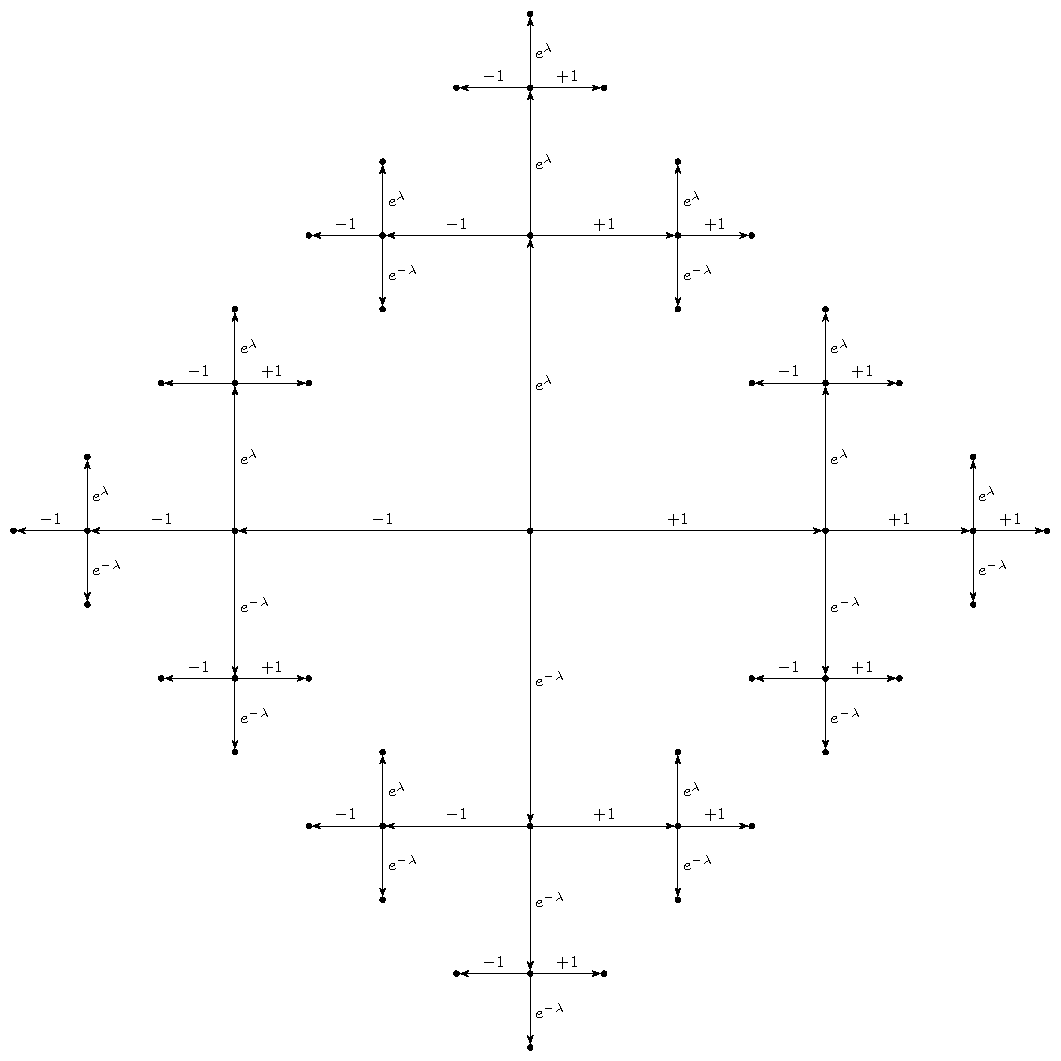
\includegraphics[width=4in]{images/cayley_i}
\caption{$\mu=1$ 时的 $\mathcal{S}^i$的生成图}
\end{figure}

生成图是四阶凯莱树。

\subsection{语法结构 $\mathcal{S}^d$}\label{subsec:syntactical}

如果我们可以引入加乘的分配律,我们可以考虑另外一种语法构造。

可以有多种典范形式。第一种典范形式是利用分配律,先加后乘或者先乘后加。
$$
0 a_1 a_2 \cdots a_n = \prod_{i} p_i \cdot \sum_{j} q_j
$$

或者

$$
0 a_1 a_2 \cdots a_n = \sum_{i} q_i + \prod_{j} p_j
$$

\begin{figure}[ht]
\centering
\resizebox{0.9\textwidth}{!}{
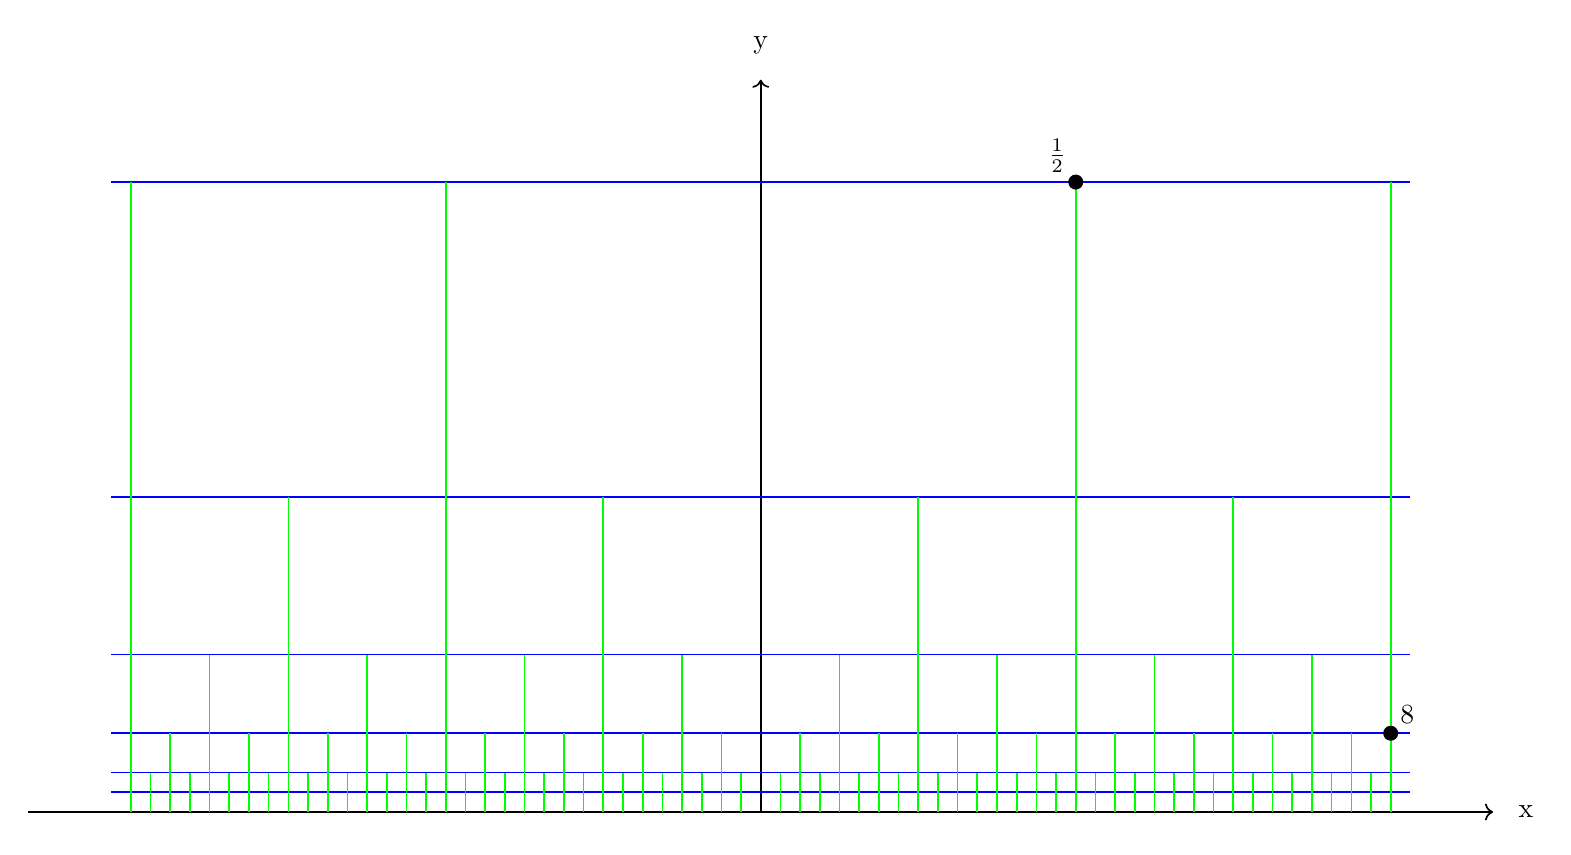
\begin{tikzpicture}
\draw [black, line width=0.6pt, ->] (0,0) to[out=90,in=270] (0,9.3);
\node [anchor=south] at (0,9.5) {y};
\draw [black, line width=0.6pt, ->] (-9.3,0) to[out=0,in=180] (9.3,0);
\node [anchor=west] at (9.5,0) {x};

\draw [blue, line width=0.6pt] (-8.25,0.25) to[out=0,in=180] (8.25,0.25);
\draw [blue, line width=0.6pt] (-8.25,0.5) to[out=0,in=180] (8.25,0.5);
\draw [blue, line width=0.6pt] (-8.25,1) to[out=0,in=180] (8.25,1);
\draw [blue, line width=0.6pt] (-8.25,2) to[out=0,in=180] (8.25,2);
\draw [blue, line width=0.6pt] (-8.25,4) to[out=0,in=180] (8.25,4);
\draw [blue, line width=0.6pt] (-8.25,8) to[out=0,in=180] (8.25,8);
\draw [green, line width=0.6pt] (-8,0) to[out=90,in=270] (-8,8.00);
\draw [green, line width=0.6pt] (-7.75,0) to[out=90,in=270] (-7.75,0.50);
\draw [green, line width=0.6pt] (-7.5,0) to[out=90,in=270] (-7.5,1.00);
\draw [green, line width=0.6pt] (-7.25,0) to[out=90,in=270] (-7.25,0.50);
\draw [green, line width=0.6pt] (-7,0) to[out=90,in=270] (-7,2.00);
\draw [green, line width=0.6pt] (-6.75,0) to[out=90,in=270] (-6.75,0.50);
\draw [green, line width=0.6pt] (-6.5,0) to[out=90,in=270] (-6.5,1.00);
\draw [green, line width=0.6pt] (-6.25,0) to[out=90,in=270] (-6.25,0.50);
\draw [green, line width=0.6pt] (-6,0) to[out=90,in=270] (-6,4.00);
\draw [green, line width=0.6pt] (-5.75,0) to[out=90,in=270] (-5.75,0.50);
\draw [green, line width=0.6pt] (-5.5,0) to[out=90,in=270] (-5.5,1.00);
\draw [green, line width=0.6pt] (-5.25,0) to[out=90,in=270] (-5.25,0.50);
\draw [green, line width=0.6pt] (-5,0) to[out=90,in=270] (-5,2.00);
\draw [green, line width=0.6pt] (-4.75,0) to[out=90,in=270] (-4.75,0.50);
\draw [green, line width=0.6pt] (-4.5,0) to[out=90,in=270] (-4.5,1.00);
\draw [green, line width=0.6pt] (-4.25,0) to[out=90,in=270] (-4.25,0.50);
\draw [green, line width=0.6pt] (-4,0) to[out=90,in=270] (-4,8.00);
\draw [green, line width=0.6pt] (-3.75,0) to[out=90,in=270] (-3.75,0.50);
\draw [green, line width=0.6pt] (-3.5,0) to[out=90,in=270] (-3.5,1.00);
\draw [green, line width=0.6pt] (-3.25,0) to[out=90,in=270] (-3.25,0.50);
\draw [green, line width=0.6pt] (-3,0) to[out=90,in=270] (-3,2.00);
\draw [green, line width=0.6pt] (-2.75,0) to[out=90,in=270] (-2.75,0.50);
\draw [green, line width=0.6pt] (-2.5,0) to[out=90,in=270] (-2.5,1.00);
\draw [green, line width=0.6pt] (-2.25,0) to[out=90,in=270] (-2.25,0.50);
\draw [green, line width=0.6pt] (-2,0) to[out=90,in=270] (-2,4.00);
\draw [green, line width=0.6pt] (-1.75,0) to[out=90,in=270] (-1.75,0.50);
\draw [green, line width=0.6pt] (-1.5,0) to[out=90,in=270] (-1.5,1.00);
\draw [green, line width=0.6pt] (-1.25,0) to[out=90,in=270] (-1.25,0.50);
\draw [green, line width=0.6pt] (-1,0) to[out=90,in=270] (-1,2.00);
\draw [green, line width=0.6pt] (-0.75,0) to[out=90,in=270] (-0.75,0.50);
\draw [green, line width=0.6pt] (-0.5,0) to[out=90,in=270] (-0.5,1.00);
\draw [green, line width=0.6pt] (-0.25,0) to[out=90,in=270] (-0.25,0.50);
\draw [green, line width=0.6pt] (0.25,0) to[out=90,in=270] (0.25,0.50);
\draw [green, line width=0.6pt] (0.5,0) to[out=90,in=270] (0.5,1.00);
\draw [green, line width=0.6pt] (0.75,0) to[out=90,in=270] (0.75,0.50);
\draw [green, line width=0.6pt] (1,0) to[out=90,in=270] (1,2.00);
\draw [green, line width=0.6pt] (1.25,0) to[out=90,in=270] (1.25,0.50);
\draw [green, line width=0.6pt] (1.5,0) to[out=90,in=270] (1.5,1.00);
\draw [green, line width=0.6pt] (1.75,0) to[out=90,in=270] (1.75,0.50);
\draw [green, line width=0.6pt] (2,0) to[out=90,in=270] (2,4.00);
\draw [green, line width=0.6pt] (2.25,0) to[out=90,in=270] (2.25,0.50);
\draw [green, line width=0.6pt] (2.5,0) to[out=90,in=270] (2.5,1.00);
\draw [green, line width=0.6pt] (2.75,0) to[out=90,in=270] (2.75,0.50);
\draw [green, line width=0.6pt] (3,0) to[out=90,in=270] (3,2.00);
\draw [green, line width=0.6pt] (3.25,0) to[out=90,in=270] (3.25,0.50);
\draw [green, line width=0.6pt] (3.5,0) to[out=90,in=270] (3.5,1.00);
\draw [green, line width=0.6pt] (3.75,0) to[out=90,in=270] (3.75,0.50);
\draw [green, line width=0.6pt] (4,0) to[out=90,in=270] (4,8.00);
\draw [green, line width=0.6pt] (4.25,0) to[out=90,in=270] (4.25,0.50);
\draw [green, line width=0.6pt] (4.5,0) to[out=90,in=270] (4.5,1.00);
\draw [green, line width=0.6pt] (4.75,0) to[out=90,in=270] (4.75,0.50);
\draw [green, line width=0.6pt] (5,0) to[out=90,in=270] (5,2.00);
\draw [green, line width=0.6pt] (5.25,0) to[out=90,in=270] (5.25,0.50);
\draw [green, line width=0.6pt] (5.5,0) to[out=90,in=270] (5.5,1.00);
\draw [green, line width=0.6pt] (5.75,0) to[out=90,in=270] (5.75,0.50);
\draw [green, line width=0.6pt] (6,0) to[out=90,in=270] (6,4.00);
\draw [green, line width=0.6pt] (6.25,0) to[out=90,in=270] (6.25,0.50);
\draw [green, line width=0.6pt] (6.5,0) to[out=90,in=270] (6.5,1.00);
\draw [green, line width=0.6pt] (6.75,0) to[out=90,in=270] (6.75,0.50);
\draw [green, line width=0.6pt] (7,0) to[out=90,in=270] (7,2.00);
\draw [green, line width=0.6pt] (7.25,0) to[out=90,in=270] (7.25,0.50);
\draw [green, line width=0.6pt] (7.5,0) to[out=90,in=270] (7.5,1.00);
\draw [green, line width=0.6pt] (7.75,0) to[out=90,in=270] (7.75,0.50);
\draw [green, line width=0.6pt] (8,0) to[out=90,in=270] (8,8.00);

\node [circle, ,draw=black, fill=black, inner sep=0pt,minimum size=5pt] at (4,8) {};
\node [circle, ,draw=black, fill=black, inner sep=0pt,minimum size=5pt] at (8,1) {};
\node [anchor=south east] at (4,8) {$\frac{1}{2}$};
\node [anchor=south west] at (8,1) {$8$};

\end{tikzpicture}
}
\caption{ $\lambda=\ln2$ 和 $\mu=\frac{1}{2}$ 时的$\mathcal{S}^d$ 的图示}\label{fig:grid0}
\end{figure}

第二种典范形式,是利用分配律,把等幂的乘法项归并起来,得到一个 $\lambda$ 的多项式的形态。

$$
0 a_1 a_2 \cdots a_n = \sum_{i} k_i \mu e^{l_i \lambda} \in R
$$

\subsection{语义结构 $\mathcal{S}^\infty$}\label{subsec:semantical}

给定一个路径 $ 0 a_1 a_2 \cdots a_n $,我们可以计算这个路径最终的计算结果,这个结果是一个实数。
也即引入估值函数:
$$
\nu(0 a_1 a_2 \cdots a_n) \to R
$$

我们说两个表达式相等,当且仅当,它们的估值相等。在估值相等作为代数结构的相等关系,我们就得到语义构造。

\newpage

\section{典范形式}\label{sec:canonical}

一般而言,给定集合 $U$ 和相等关系 $=$, 典范形式是商集 $U/=$ 上的一种选出方法 $c: U/= \to U$,它从相等关系的每一类中选出一个代表,且满足如下条件

\begin{itemize}
    \item 对合 $  c(x) = c(c(x)) $
    \item 确定 $  c(x_1) = c(x_2) \iff x_1 = x_2  $
\end{itemize}

在算术表达式的上下文里,我们需要给出典范形式的清晰定义。

\subsection{表达式树与线索}



\subsection{表达式族的刻画}

\subsection{表达式的典范形式}

典范形式必须能够覆盖所有的自由生成

\newpage

\section{网格细化与完备化}\label{subsec:completeness}

\subsection{可伸缩和数位制}

先让我们做一段有启发性的思考—我们是如何理解和表达实数的呢?我们是通过比较容易把握的有理数来实现的。

有理数是对单位一的有限叠加与有限平分。如果我们改变单位一的长度,我们会发现有理结构是不变的,这种结构可伸缩的特性给数位制奠定了几何基础。

考虑一个位置测量的过程:为了测量一个未知位置,我们在某一个单位长度的基础上,用数刻画了一个大约的位置。
同一个有理结构的可伸缩性意味着,在不同长度测量单位的基础上,我们有可能可以组合不同长度单位的测量结果,用不同的数字的组合,来实现精细的测量。
假设我们的第一次测量结果是 $l_1$,第二次测量时单位一缩小了整数 $k$ 倍,那么第二次测量在 $kl$ 时,两个测试的长度是重合的。
这样的话,我们就能构造一个非常清晰的逼近测量的过程,不断把单位一缩小 $k$ 倍,获得更多的精细级别上的测量数字,然后组合不同剩余段上的测量数字,
最终获得一个数位表示。

综合以上,数位制可以被理解成为一个逼近测量的过程。下面,我们形式化地定义这个逼近测量的过程。

假设符号表为$\Sigma = \{s_i | i = 0 \cdots n\}$,针对基准点 $o$、任一点 $y$ 和某一个测量精度 $\rho$,我们有
刻度映射 $T_o^\rho: s_i \mapsto x_i$ 和某个点的辨识区域 $D^\rho: z \mapsto S_z$。
于是,我们有全体符号的辨识区域 $S_o^\rho = \bigcap_{i=0}^n (D^\rho \circ T_o^\rho)(s_i)$

首先,我们定义测量精度 $\rho$ 上的测量过程$M_o^\rho: y \mapsto s_k$,它是如下的算法过程:
\begin{itemize}
    \item 参量:基准点 $o$ 和精度 $\rho$
    \item 输入:点 $y$
    \item 输出:符号 $s_k$
    \item 过程:遍历所有的 $\{0 \cdots n\}$ 以确定 $k$ 使得$y \in (D_\rho \circ T_\rho)(s_k)$
\end{itemize}

最后需要指出,我们仍然有空间可以去思考:无限符号情况下逼近测量过程和并行算法过程的几何含义。

\subsection{网格和加细}

\subsection{完备化}

赋值 $A$ 是从 $R$ 映射到流形 $M$,加乘表达式的细密意味着 $E = E_0 \cup E_1 \cup E_2 \cup \cdots E_n$ 是一种按照细密程度的分层
从每个 $E_i$ 中取点 $x_i$ 使得 $A(x_i)$ 在流形 $M$ 上构成柯西序列,在此条件下,我们必须证明 $x_i$ 在代数上的收敛性。
也即,如果度量上的收敛性蕴涵代数上的收敛性,我们称赋值 A 是完备的。

\subsection{赋值、网格和典范形式}

如何从一个合适的流形赋值得到网格和典范形式

什么是合适的赋值

\newpage

\section{深入流方程}

\subsection{拉回}

\begin{figure}[ht]
\centering
\begin{tikzpicture}

\filldraw [black] (4,1) circle (2pt) node[align=center, below] {$\alpha$};
\filldraw [black] (2,3) circle (0pt) node[align=center, above] {$\nu^{-1}(f^1)$};
\filldraw [black] (7,3) circle (0pt) node[align=center, above] {$\nu^{-1}(f^2)$};
\draw [gray] (0,0) to[out=300,in=240] (4,1);
\draw [->] (4,1) to[out=120,in=300] (2,3);
\draw [->] (4,1) to[out=30,in=240] (7,3);

\draw [->] (3.5,-0.5) to[out=270,in=90] (3.5,-5);
\filldraw [gray] (3.8,-3) circle (0pt) node[align=center, below] {$\nu$};

\filldraw [gray] (3.5,-5.5) circle (2pt) node[align=center, below] {$x_0 = \nu(\alpha)$};
\filldraw [gray] (3.5,-6.5) circle (2pt) node[align=center, below] {$x_0$};
\filldraw [gray] (3.5,-7.5) circle (2pt) node[align=center, below] {$x_0$};
\draw [gray] (0,-5.5) to[out=0,in=180] (7,-5.5);
\draw [->] (3.5,-6.5) to[out=0,in=180] (4.5,-6.5);
\draw [->] (3.5,-7.5) to[out=0,in=180] (5.5,-7.5);
\filldraw [gray] (1.0,-6.2) circle (0pt) node[align=center, below] {$f^1 = x_0 + \mu t$};
\filldraw [gray] (1.0,-7.2) circle (0pt) node[align=center, below] {$f^2 = x_0 e^{\lambda t}$};
\filldraw [gray] (7.0,-6.2) circle (0pt) node[align=center, below] {$\dot{f}^1 = \mu$};
\filldraw [gray] (7.0,-7.2) circle (0pt) node[align=center, below] {$\dot{f}^2 = \lambda x_0$};

\end{tikzpicture}
\caption{拉回}
\end{figure}

\subsection{等值线与梯度}

从流方程很容易导出局部坐标系下的等值线方程

\begin{equation}
    \mu \cos \theta_c + a \lambda \sin \theta_c = 0
\end{equation}

于是有

\begin{equation}
    \theta_c = - \arctan \frac{\mu}{a \lambda}
\end{equation}

等值线和梯度是联系在一起的,两者彼此垂直

\begin{equation}
    \theta_g = \pm \frac{\pi}{2} - \arctan \frac{\mu}{a \lambda}
\end{equation}

于是沿着 $\theta_g$ 我们可以取到

\begin{equation}
    \frac{da}{ds} = \mu \cos (\pm \frac{\pi}{2} - \arctan \frac{\mu}{a \lambda}) + a \lambda \sin (\pm \frac{\pi}{2} - \arctan \frac{\mu}{a \lambda})
\end{equation}

\begin{equation}
    \frac{da}{ds} = \pm \sqrt {\mu^2 + a^2 \lambda^2} \label{eq:gradient}
\end{equation}

方程 \eqref{eq:gradient} 可解,得出沿着梯度流线 $a$ 和 $s$ 的关系如下:

\begin{equation}
    \pm s = \frac{1}{\lambda} \ln \frac{\mu}{a + \sqrt{\mu^2 + \lambda^2 a^2}} + c
\end{equation}

如果约定 $\mu > 0, \lambda >0, s >= 0$ 且 $s = 0$ 时有 $a = 0$ 公式还可以进一步变形,得到

\begin{equation}
    a = \frac{\mu}{\lambda^2 - 1} (- e^{\lambda s} + \sqrt{\lambda^2  e^{2 \lambda s} - \lambda^2 + 1})
\end{equation}

\subsection{梯度-等值线坐标系}

在梯度方向的基础上按右手螺旋引入转角 $\phi$,我们建立梯度-等值线为参照的局部极坐标系,有沿转角 $\phi$ 移动时 $a$ 的增长率为

\begin{equation}
    \frac{da}{ds} = \mu \cos (\frac{\pi}{2} - \arctan \frac{\mu}{a \lambda} + \phi) + a \lambda \sin (\frac{\pi}{2} - \arctan \frac{\mu}{a \lambda} + \phi)
\end{equation}

化简得到

\begin{equation}
    \frac{da}{ds} = \sqrt {\mu^2 + a^2 \lambda^2} \cos \phi\label{eq:contourgradient}
\end{equation}

也就是梯度-等值线坐标系下的流方程。

\subsection{火烧法}

\subsubsection{赋值例六}\label{subsec:exmp6}

\begin{figure}[ht]
\centering
\begin{tikzpicture}
    \tkzDefPoint(-4,0){O1}
    \tkzDefPoint(0,0){O}
    \tkzDefPoint(4,0){O2}

    % with K=2 we search some points like I such as IA=2 IB
    \tkzDefCircle[apollonius,K=2](O1,O2) \tkzGetPoint{K1}
    % K1 is the center of the circle
    \tkzGetLength{rAp} % we get also the radius

    draw [name path=O1--O2] ($\Omega_1$) -- ($\Omega_2$);

\end{tikzpicture}
\caption{伪圆坐标系}\label{fig:horocyclecoord}
\end{figure}



\subsection{几个问题}

在一种典范形式的几何上,能否表示所有的表达式?在一种典范形式的几何上,其他典范形式体现为什么?

调和映照、狄利克莱能量、极小曲面

关系的视角:逻辑、复杂性都来源于极小曲面,极小曲面间的映照

\newpage

\subsection{变换与管型构造}
\newpage

\section{赋值与流形}

\subsection{给定赋值的情形}

\subsection{给定流形的情形}

\newpage

\section{紧化的算术意义}

欧拉的著名等式

\subsection{几何上的紧化}

\subsection{紧化与算术}

\subsection{不停机程序}

\newpage

\section{走向更一般的表示}

\subsection{抛弃数的特殊性}

拥抱表达式,摆脱数

\subsection{函数的表示}

\newpage

\section{回到黎曼}

\subsection{有何不同}

\subsection{四阶无限边形镶嵌}

\subsection{黏合零线}

\subsection{管型构造}

\newpage

\section{最后的陈词}

本节给出我们的一些观察和遐想。

\subsection{引向复杂性?}

我们已经验算了一些例子,这些例子的赋值是 Laplace 算子的特征向量,为什么会这样呢?
我们还没有解决这个问题,但有一些有趣的观察。我们知道,大数乘法的快速算法需要用 FFT 做变换。
而 FFT 是调和分析的一种技术,它天然和 Laplace 算子的特征向量有关系。

有没有可能 Laplace 算子出现在这里,是因为表达式的几何空间和两种复杂性有内在的联系?
在计算的时间复杂度和表征的空间复杂度的相互作用下,算术表达式的典范形式类似一张缓缓展开的极小曲面。

\subsection{分析的新语言}

我们有两种方式使用一个计算机程序。一种是使用它的最终效果,一种是使用它的计算过程。
前者的例子是程序库的各种标准例程,比如 $\sin$、$\cos$ 等等,我们不在乎它的实现细节和计算的中间状态,只在乎最终结果。
后者的例子是打游戏,游戏程序循环的每一步,都导致我们用户在音视频上的某种体验,整个计算过程都是我们需要的。

以上两种机制也同样出现在算术表达式的空间里,可以帮助我们定义函数。计算过程是空间里的一条路径,这条路径本身定义了一个演化函数。
而路径头尾两端的值的差异,就是这个计算过程的效果。如果我们改变头部的输入值,不改变相对的计算路径,那么可以预期输出也会改变。
这样基于计算路径头尾两端的差异,我们也可以定义函数。

经典的分析学是建立在函数的语言上的,但我们仍然能看到它和算术的对应关系。微分是局部的差,而积分对应的是累加。如果累加对应经典的积分,
那么累积加和乘得到的是什么呢?

更有趣的是,计算路径头尾两端差异的思路,其实暗含了微积分基本定理、Stokes公式、Gauss-Bonnet定理这一条发展线索。
有可能我们可以发展新的分析学的语言,来重写古典的结论。

\subsection{科学史的考察}

追寻计算机科学的由来,我们会发现它的源头来自 19 世纪非欧几何的发现和数学分析的严密化。
当时人们想弄清楚这些新数学的基础,经过几代数学家不断努力,在 19 世纪末,人们认为数学基础可以通过算术化和形式化,得到一个完美解决。
但这个思路很快被哥德尔的工作否定了。并在此基础上,诞生了计算机科学。

哥德尔的思想蕴涵着开放世界的丰富,和这个世纪火热的学习话题遥遥相对。
但在这里,我想问另外一个问题,从几何和分析里衍生出来的计算机科学,现在离几何、分析那么遥远,这在科学史上是正确的一种状态吗?

人们常说,数和形是数学的基本主题。让我们看一下数的早期历史。
从石器时代非洲的骨刻,我们可以看到数的概念表征和计算过程是浑然一体的,这种表征非常繁琐,计算的能力也非常有限。
其后,数的表征,经过古埃及的不成熟形态,到达了古巴比伦的数位制。

在这个历史过程里,人们遗忘了一个隐藏的巨大世界—那就是表达式,或者说计算过程。
数作为一种表征,本来就是计算过程的高度凝练的表达,但它一旦符号化后,就成为我们追求的目标。
于是,我们往往关注计算过程的结果,而忽视了过程本身蕴含的众多信息。

过程比结果更重要。我们找到了计算过程的另外一种几何表征,它会极大的提升我们的能力。
它有潜力可以把分离的几何、分析和计算这三个学科重新黏合在一起。

\begin{itemize}
    \item 几何:算术表达式的几何化得到一个流形
    \item 分析:流形上的路径本质上是一种特殊的积分
    \item 计算:Laplacian 的出现有一种潜在的计算复杂性的解释
\end{itemize}

虽然这个几何化本身不涉及学习问题,但它能为当下的学习问题开辟一些新的分析视角。

在目前的计算机科学里,人们大多讨论停机的程序。停机程序,我们可以清晰定义它的作用,从而容易分析这一类程序的性质。
然而 1996 年有论文论述了停机问题的可学习性。这意味着,学习过程的背后还有丰富的内涵可供研究。

在算术表达式几何化的框架里,函数会以效果和过程两种形态呈现,效果的考察方式就对应了停机程序,
而过程的考察方式可以包括不停机程序。比如,我们可以分析计算路径在几何的无穷边界处的性态;
也可以通过随机游走的方式,重新把 Chaitin 的 AIT 理论引入。

我们有理由相信,算术表达式的几何化是一个新变革的开端。

\subsection{无尽的遐想}

\newpage
\phantomsection
\addcontentsline{toc}{section}{参考文献}
\bibliographystyle{ieeetr}
\bibliography{biblio/article}

\newpage
\appendix

\section{推导}

\begin{equation}
    \pm s = \frac{1}{\lambda} \ln \frac{\mu}{a + \sqrt{\mu^2 + \lambda^2 a^2}} + c
\end{equation}

或者进一步变形,得到

\begin{equation}
    \mu e^{c \mp \lambda s} = a + \sqrt{\mu^2 + \lambda^2 a^2}
\end{equation}

进一步得到

\begin{equation}
    a^2 + \mu^2 e^{2 c \mp 2 \lambda s} - 2 a \mu e^{c \mp \lambda s} = \mu^2 + \lambda^2 a^2
\end{equation}

\begin{equation}
    (\lambda^2 - 1)a^2 + 2 a \mu e^{c \mp \lambda s} - \mu^2 (e^{2 c \mp 2 \lambda s} - 1) = 0
\end{equation}

\begin{equation}
     4 \mu^2 e^{2c \mp 2 \lambda s} + 4 (\lambda^2 - 1) \mu^2 (e^{2 c \mp 2 \lambda s} - 1)
\end{equation}

\begin{equation}
     4 \mu^2 e^{2c \mp 2 \lambda s} + 4 (\lambda^2 - 1) \mu^2 e^{2 c \mp 2 \lambda s} - 4 (\lambda^2 - 1) \mu^2
\end{equation}

\begin{equation}
     4 \lambda^2 \mu^2 e^{2 c \mp 2 \lambda s} - 4 \lambda^2 \mu^2 + 4 \mu^2
\end{equation}

\begin{equation}
     4 \mu^2 (\lambda^2  e^{2 c \mp 2 \lambda s} - \lambda^2 + 1)
\end{equation}

\begin{equation}
    (\lambda^2 - 1)a^2 + 2 \mu e^{c \mp \lambda s} a - \mu^2 (e^{2 c \mp 2 \lambda s} - 1) = 0
\end{equation}

\begin{equation}
    a = \frac{- 2 \mu e^{c \mp \lambda s} \pm 2 \mu \sqrt{\lambda^2  e^{2 c \mp 2 \lambda s} - \lambda^2 + 1}}{2(\lambda^2 - 1)}
\end{equation}

\begin{equation}
    a = \frac{- \mu e^{c \mp \lambda s} \pm \mu \sqrt{\lambda^2  e^{2 c \mp 2 \lambda s} - \lambda^2 + 1}}{\lambda^2 - 1}
\end{equation}

\begin{equation}
    a = \frac{\mu }{\lambda^2 - 1} (- e^{c \mp \lambda s} \pm \sqrt{\lambda^2  e^{2 c \mp 2 \lambda s} - \lambda^2 + 1})
\end{equation}

\begin{equation}
    a = \frac{\mu }{\lambda^2 - 1} (- e^{\lambda s} + \sqrt{\lambda^2  e^{2 \lambda s} - \lambda^2 + 1})
\end{equation}

\end{document}


